% Documento principal
\documentclass[10pt]{book}

% Pacotes necessários
\usepackage[landscape, top=5mm, left=10mm, right=10mm, bottom=0mm, paperwidth=118mm, paperheight=210mm]{geometry}  % Configuração da página
\usepackage{fancyhdr}  % Para configuração de cabeçalhos e rodapés
\usepackage{multicol}  % Para uso de múltiplas colunas
\usepackage{enumitem}  % Para personalizar listas
\usepackage{xcolor}    % Para uso de cores
\usepackage{graphicx}  % Para manipulação de gráficos
\usepackage{hyperref}  % Para links clicáveis
\usepackage{csvsimple} % Para tabelas openCSV
\usepackage{expl3}		% Para matemática avançada
\usepackage{pgffor}  % Para funções de programação
\usepackage{array}  % Tabelas em LaTeX com controle avançado de colunas.
\usepackage{wasysym}
\usepackage[brazil]{babel}  % Configuração do idioma para português do Brasil
\usepackage[utf8]{inputenc}  % Configuração da codificação de entrada

% Pacotes para suporte ao BibTeX
\usepackage[num]{abntex2cite}  % Estilo ABNT para citações
\usepackage{babelbib}  % Suporte ao idioma no BibTeX

% Configuração do estilo da página
\pagestyle{fancy}
\fancyhead[L]{ABC da Inform\'{a}tica}
\fancyfoot[C]{\LaTeX}
\fancyhead[R]{Alexandre Aravecchia}
\fancyfoot[R]{\thepage}
\renewcommand{\headrulewidth}{1pt}
\renewcommand{\footrulewidth}{1pt}

% Configuração de dimensões
\setlength{\headsep}{5mm}
\setlength{\headheight}{7.5mm}
\setlength{\footskip}{-5mm}
\setlength{\textheight}{92.5mm}
\setlength{\topmargin}{-25mm}
\setlength{\columnsep}{5mm}
\setlength{\parskip}{1mm plus 5mm}

% Carregar a fonte OpenSans
\usepackage[default,scale=0.95]{opensans}

% Definição de cores
\definecolor{black}{rgb}{0,0,0}
\definecolor{white}{rgb}{1,1,1}
\definecolor{linkblue}{rgb}{0,0,0.7}  % Cor azul para os links

% Configurações do pacote hyperref
\hypersetup{
	colorlinks=true,
	linkcolor=linkblue,
	filecolor=linkblue,
	urlcolor=linkblue,
	citecolor=linkblue,
	pdfborder={0 0 0},  % Remove a moldura dos links
}

% Informações do título
\title{
	\vspace*{-5mm}
	\resizebox{60mm}{12mm}{\textcolor{black}{ABC}}
	\\
	\resizebox{60mm}{6mm}{\textcolor{black}{\textbf{da Inform\'{a}tica}}}
	\\
	\resizebox{80mm}{5mm}{\textcolor{black}{Aulas Expositivas}}
}
\author{
	\resizebox{60mm}{4mm}{\textcolor{black} Alexandre Aravecchia}
}
\date{\small \today}

% Início do documento
\begin{document}
	
	% Gera o título
	\maketitle
	
	% Cria uma tabela de conteúdo em duas colunas
	\begin{multicols}{2}
		\tableofcontents
	\end{multicols}
	
	% Adiciona a citação com link clicável
	{\normalsize Fonte: \href{URL_DA_FONTE}{Nome da Fonte}}
	
	% Inclui o conteúdo dos capítulos a partir de um arquivo externo
	%	Bora lá?

Somos eu e você, professora, colegas de trabalho, geralmente amigos, e muitas vezes até parentes, então podemos ser sinceros?

O que vou dizer é constrangedor, mas, pergunte a uma criança de 8 anos se ela gosta da escola.

No fundo ela dirá que não, e saberá por quê. Não discuta, ou você irá perder.

Pergunte a ela oq ela não gosta na escola, e você terá um vislumbre do quê é ter 8 anos numa escola publica.

%\end{multicols}

\color{black}

	\chapter[\large Apresentação]{Apresentação}

	\begin{multicols}{2}
{\small	Alô meninos e meninas!

Eu sou o Alexandre Aravecchia, designer, desenvolvedor, professor de computação, nerd convito, fui diagnosticado com altas habilidades) ainda na escola primária, eu sou nerd mesmo, raiz!, e, como muitos de vocês, eu sou um sobrevivente.

Eu quero falar uma coisa importante prá vocês, que pode parecer meio óbvia, mas gente \textbf{filha da puta} existe em todo lugar, infelizmente.

Em casa, na família, no trabalho, na escola, na igreja, no círculo de amizades, ao longo de toda sua vida, não é a maioria, mas sempre nós vamos ter que lidar com pessoas que não querem nada além de ver o nosso pescoço pendurado numa forca, ou de preferência numa prisão, onde esta pessoa é o carcereiro e você não consegue sair, por mais que você tente ou se esforce prá fazer tudo bonitinho...

Sempre vai estar faltando alguma coisa práquele tão sonhado prêmio prometido, não é assim?

Você sabe que é.

Acontece que existe uma brecha aí nessa prisão, que o carcereiro esqueceu de fechar, e neste trabalho eu quero mostrar pra vocês uma saída prá essa armadilha.

Curto e grosso:

É a gaiola financeira a primeira coisa que um narcisista vai utilizar contra você, afinal, abra seus olhos:

Ele está sempre em posição de superioridade frente a você, tanto socialmente quanto financeiramente: seja uma mãe ou um pai narcisistas, um marido abusivo ou um chefe aproveitador, ele geralmente é quem manda, e na maior parte do tempo usa contra você uma coisa que ele tem, e você não: dinheiro!

Dentre todas as armadilhas narcisistas que nós podemos cair, acho que a pior de todas é a financeira.

Pense comigo: sem uma colocação profissional, um emprego, um trabalho que coloque dinheiro na tua conta todo mês, como você vai fazer para fugir do cativeiro, e estabelecer o tão sonhado contato zero? Morando na rua?

Acho que não é boa idéia!

Como vai conseguir fazer uma terapia, então? Mesmo que consiga pelo SUS, vocês acham que o narcisista vai deixar você ir assim, sem infernizar sua vida até que você desista?

Então, ao invés de dizer para você trabalhar duro ou lutar como uma fera, para conseguir só ser acorrentado mais e mais, proponho uma coisa: ao invés de trabalhar duro, vamos desta vez usar a cabeça!

Sigam-me os bons!
}
\vfill\null
\pagebreak

\end{multicols}
	
	\large
\begin{multicols}{2}
	A ideia do Código Viking é ser a base \LaTeX \space de trabalho para qualquer professor, tanto para organizar seu plano de trabalho, como para preparar suas aulas, escrever seus livros e artigos, ou desenvolver suas palestras, de forma rápida, fácil, com uma diagramação perfeita, digna de um bom professor.

Assim, surgiu também a idéia do \textbf{Sistema Efestus}, que incorpora scripts Shell e Python ao sistema operacional, para disponibilizar o plano de aulas numa rede local e organizar o trabalho nos Laboratórios de Informática, em escolas públicas de todo o Brasil.

Ja o \textbf{ABC da Informática} é um plano de aulas pessoal, meu, que incorporei a este documento, como exemplo do funcionamento do Código Viking, e para testar o Sistema Hefestus em sala de aula.

Você pode utilizá-lo a vontade, para fins não comerciais, como ponto de partida para criar seu próprio plano de aulas ou gerenciar o Laboratório da sua escola.

Sinta-se à vontade para enviar dúvidas ou sugestões para aravecchia@gmail.com.

Copie, modifique (mantendo os direitos autorais), divulgue e compartilhe!

\vfill\null
\columnbreak

\subsection[Preâmbulo]{Preâmbulo}

\lstinputlisting[basicstyle=\ttfamily, style=LaTeXStyle, label=lst:LaTeXCode]{./HEFESTUS.tex}

\vfill
\columnbreak

\subsection[Capítulo]{Capítulo}

\lstinputlisting[style=LaTeXStyle, label=lst:LaTeXCode]{./CAPITULOS-HEFESTUS.tex}

\subsection[Pacote Listings para códigos-fonte]{Pacote Listings para códigos-fonte}

\begin{verbatim}
	\lstinputlisting[style=LaTeXStyle, label=lst:ArduinoCode]
	{./TeX-git/ARDUINO-CODE.tex}

\lstinputlisting[style=LaTeXStyle, label=lst:ShellCode]
{./TeX-git/SHELL-CODE.tex}

\lstinputlisting[style=LaTeXStyle, label=lst:LaTeXCode]
{./TeX-git/LATEX-CODE.tex}

\lstinputlisting[style=LaTeXStyle, label=lst:LaTeXCode]
{./TeX-git/PYTHON-CODE.tex}
\end{verbatim}

\subsection[Exemplos de códigos-fonte em pacote Listings]{Exemplos de códigos-fonte em pacote Listings}


\lstinputlisting[style=ArduinoStyle, label=lst:ArduinoCode]
{./TeX-git/Arduino-CODE.tex}

\lstinputlisting[style=C, label=lst:CCode]
{./TeX-git/C-CODE.tex}

\lstinputlisting[style=LaTeXStyle, label=lst:LaTeXCode]
{./TeX-git/LaTeX-CODE.tex}

\lstinputlisting[style=PythonStyle, label=lst:PythonCode]
{./TeX-git/Python-CODE.tex}

\end{multicols}

\vfill\null
\pagebreak


	
		Professor, designer industrial, catequizador Linux, pioneiro do 3d no BR.

\vfill\null
\pagebreak

	
	\section[Por quê aprender computação?]{Por quê aprender computação?}
	Porque estamos no século 21, oras!

Quase tudo o que fazemos, hoje, de alguma forma envolve computadores e internet.

Senão, vejamos:

Para estudar...
\vfill\null
\pagebreak


	
	\section[Mas e o curso que eu fiz?]{Mas e o curso que eu fiz?}
		\vfill\null
\pagebreak


	
	\section[E o quê este curso tem de diferente?]{E o quê este curso tem de diferente?}
\vfill\null
\pagebreak


	
	\section[Como a computação pode me ajudar?]{Como a computação pode me ajudar?}
\vfill\null
\pagebreak


	
	\section[Preciso pagar alguma coisa?]{Preciso pagar alguma coisa?}
\vfill\null
\pagebreak



	\chapter[\large O computador]{O computador}
	
		\section[O que é um computador]{O que é um computador}
	\vfill\null
\pagebreak
{\Huge Computador\\}

{\LARGE do latim \textit{computare}:\\

“calcular, estimar, somar, contar”,\\

{\Large de COM-PUTARE, “junto” + “calcular, avaliar, estimar”.\\}

{\LARGE O computador é uma grande calculadora.}

\vfill
\pagebreak

{\LARGE Mas ele também é ótimo para colocar as coisas em \textbf{ordem}.\\}

{\Large no francês: \textit{\textbf{ordinateur}}
	
{\Large no italiano: \textit{\textbf{ordenatore}} (ordenador)\\
		
	\vfill
	\pagebreak

\begin{center}
	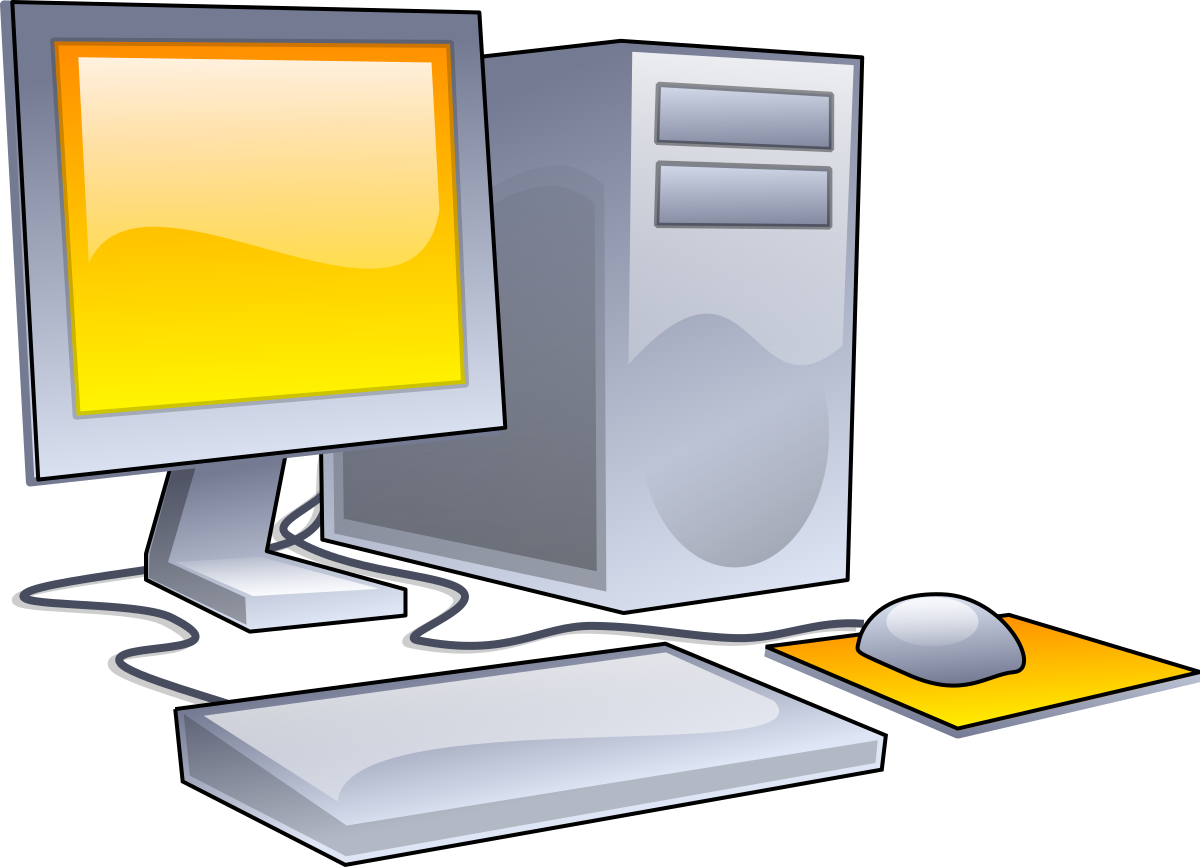
\includegraphics[height=\textheight]{./IMG/Desktop_computer_clipart_-_Yellow_theme.svg.png}
\end{center}

	\vfill
\pagebreak

\begin{center}
	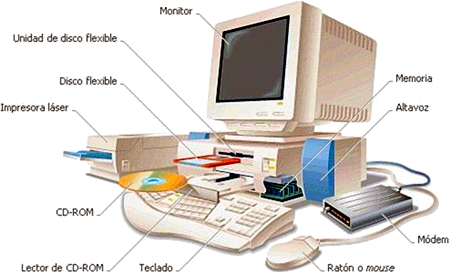
\includegraphics[height=\textheight]{./IMG/th-1517019610.jpg}
\end{center}

\vfill
\pagebreak

\begin{multicols}{3}
	
{\Large Entrada}
	
	\begin{center}
	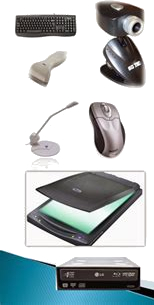
\includegraphics[height=.9\textheight]{./IMG/entrada.jpg}
\end{center}

\vfill
\columnbreak

{\Large Saida}

\begin{center}
	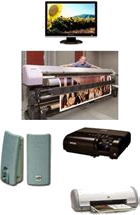
\includegraphics[height=.9\textheight]{./IMG/saida.jpg}
\end{center}

\vfill
\columnbreak

{\Large Mistos}

\begin{center}
	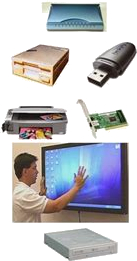
\includegraphics[height=.9\textheight]{./IMG/mistos.jpg}
\end{center}

\vfill
\pagebreak
\end{multicols}

{\large Gabinete ou torre:}
	\begin{center}
		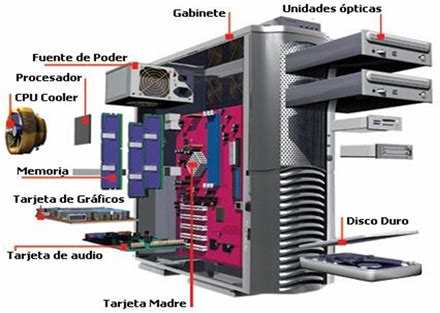
\includegraphics[height=.9\textheight]{./IMG/th-997046030.jpg}
	\end{center}

\vfill
\pagebreak

	\begin{center}
	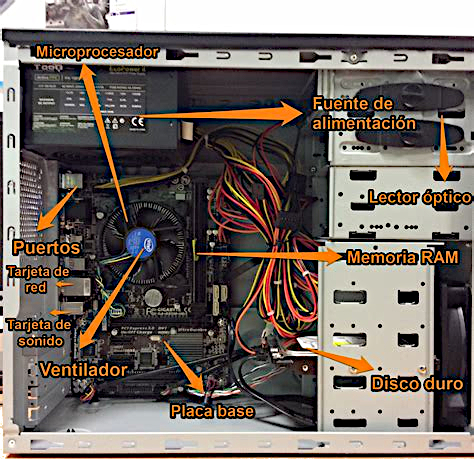
\includegraphics[height=\textheight]{./IMG/th-1583851518.jpg}
\end{center}

\vfill
\pagebreak

\begin{center}
	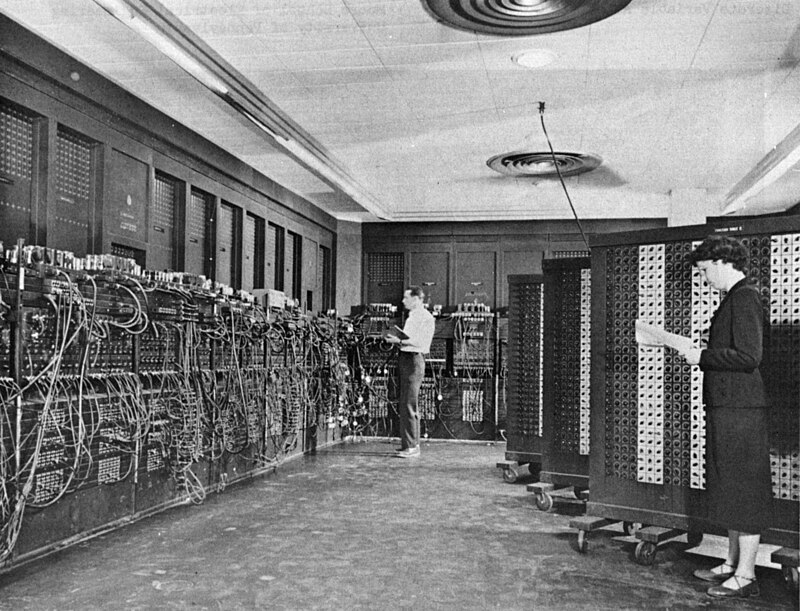
\includegraphics[height=\textheight]{./IMG/ENIAC.jpg}
\end{center}

\vfill
\pagebreak


		
	\section[Quem inventou o computador]{Quem inventou o computador}
	\vfill\null
\pagebreak


			
		\section[Senta que lá vem História!]{Senta que lá vem História!}
	\vfill\null
\pagebreak


	
	\subsection[O fogo]{O fogo}
	\vfil\null
\pagebreak


		
		\subsection[O osso de Ishangô]{O osso de Ishangô}

\begin{multicols}{2}
	{\normalsize Fonte: \href{https://pt.wikipedia.org/wiki/Osso_de_Ishango}{https://pt.wikipedia.org/wiki/Osso\_de\_Ishango}}
	
	{\large Paleolítico Superior ($\sim$20 000 - 18 000 a.C.)
	
	É um longo osso castanho (a fíbula de um babuíno) com um pedaço de quartzo afiado incrustado em uma ponta, que talvez fosse utilizado para gravar ou escrever.
}
\vfill\null
\columnbreak	

	\begin{center}
		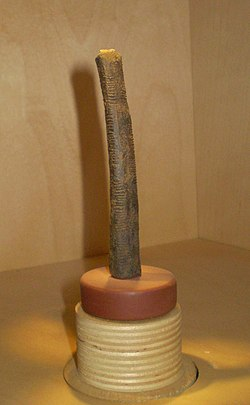
\includegraphics[height=.75\textheight]{./IMG/Os_d'Ishango_IRSNB.JPG}
	\end{center}


\begin{center}
	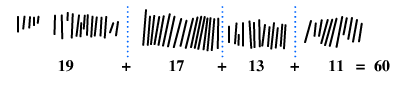
\includegraphics[width=\linewidth]{./IMG/IshangoColumnA.png}

	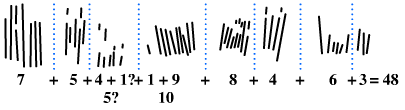
\includegraphics[width=\linewidth]{./IMG/IshangoColumnB.png}

	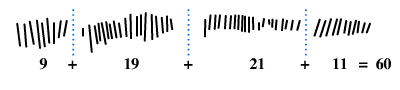
\includegraphics[width=\linewidth]{./IMG/IshangoColumnC.png}
\end{center}

\vfill
\columnbreak

	{\large Cogitou-se a princípio que era utilizado para realizar contagens, porque há uma série de traços talhados, divididos em três colunas, ao longo de todo o comprimento da ferramenta.}


\vfill\null
\pagebreak
\end{multicols}




	\subsection[O chefe da tribo]{O chefe da tribo}
\vfill\null
\pagebreak



	\subsection[O problema das cabras]{O problema das cabras}
\vfill\null
\pagebreak



	\subsection[Tabuletas de argila]{Tabuletas de argila}

\begin{multicols}{2}
\large Sumérios (Mesopotâmia, atual Iraque.)

$\sim$3500 a.C.

\vfill\null
\columnbreak

\begin{center}
	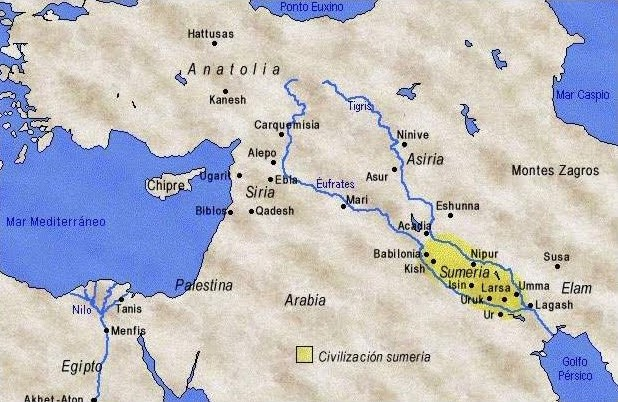
\includegraphics[width=\linewidth]{./IMG/sumeria.jpg}
\end{center}
\end{multicols}	
\vfill
\pagebreak

\begin{center}
	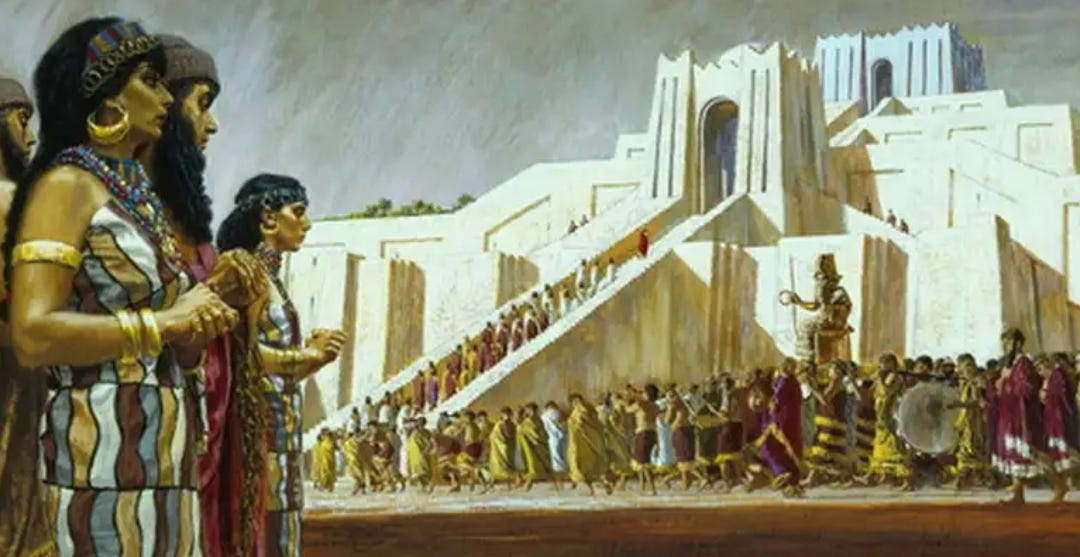
\includegraphics[width=\linewidth]{./IMG/1_62aXcnbpy4HJKcEGK0p6dQ.jpg}
\end{center}

\vfill
\pagebreak

\begin{center}
	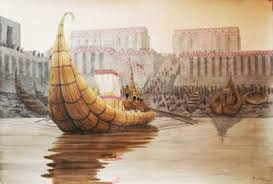
\includegraphics[width=\linewidth]{./IMG/barcos-sumerios.jpeg}
\end{center}

\vfill
\pagebreak

\begin{center}
	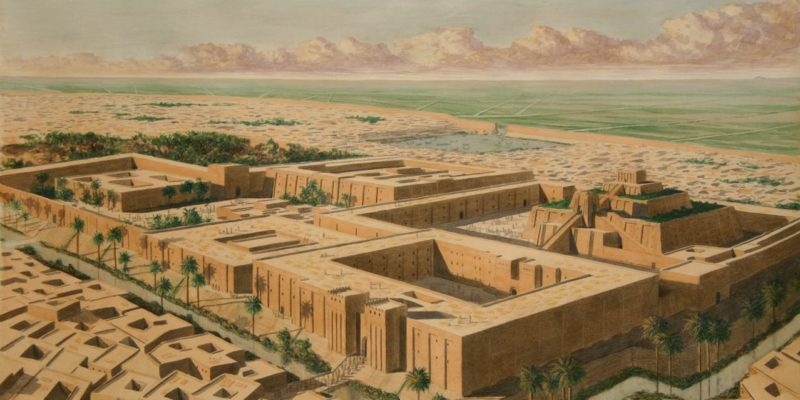
\includegraphics[width=\linewidth]{./IMG/sumerios.jpg}
\end{center}

\vfill
\pagebreak

\begin{multicols}{2}
	\begin{center}
	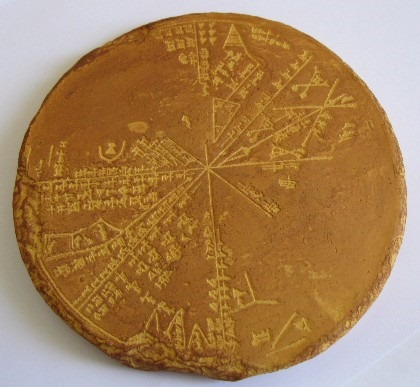
\includegraphics[width=\linewidth]{./IMG/tumblr_meje4cXeVb1qfub7eo1_500.jpg}
\end{center}

\vfill
\columnbreak

\begin{center}
	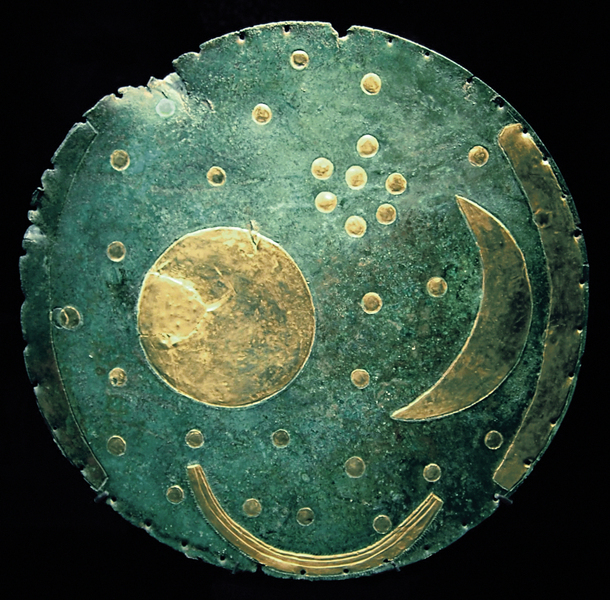
\includegraphics[width=\linewidth]{./IMG/nebra-scheibe.jpg}
\end{center}

\end{multicols}

\vfill
\pagebreak

\begin{center}
	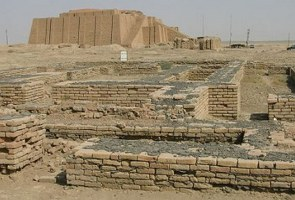
\includegraphics[width=\linewidth]{./IMG/ruinas_cidade_ur.jpg}
\end{center}

\begin{multicols}{2}

	\begin{center}
	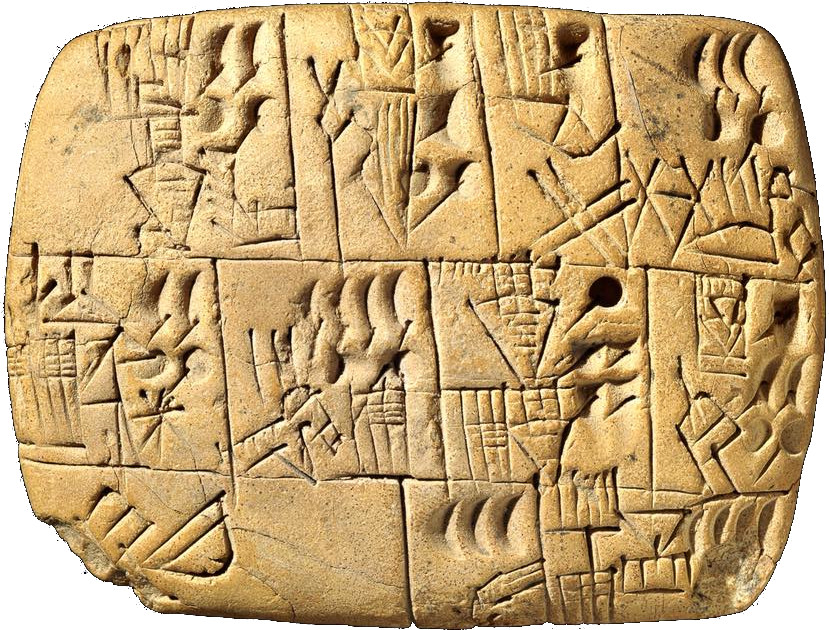
\includegraphics[width=\linewidth]{./IMG/argila.jpeg}
	\end{center}

\vfill
\columnbreak

	Formação do Estado:
\large
\begin{itemize}
	\item Quantos soldados?
	\item Quantos cavalos?
	\item Quantas espadas?
	\item Quantos bois?
	\item Quanto trigo?
	\item Quantos escravos?
	\item Quantas pessoas para alimentar?
	\item Quem deve pagar quanto de tributos?
	
\end{itemize}

	\vfill
\columnbreak
\begin{center}
	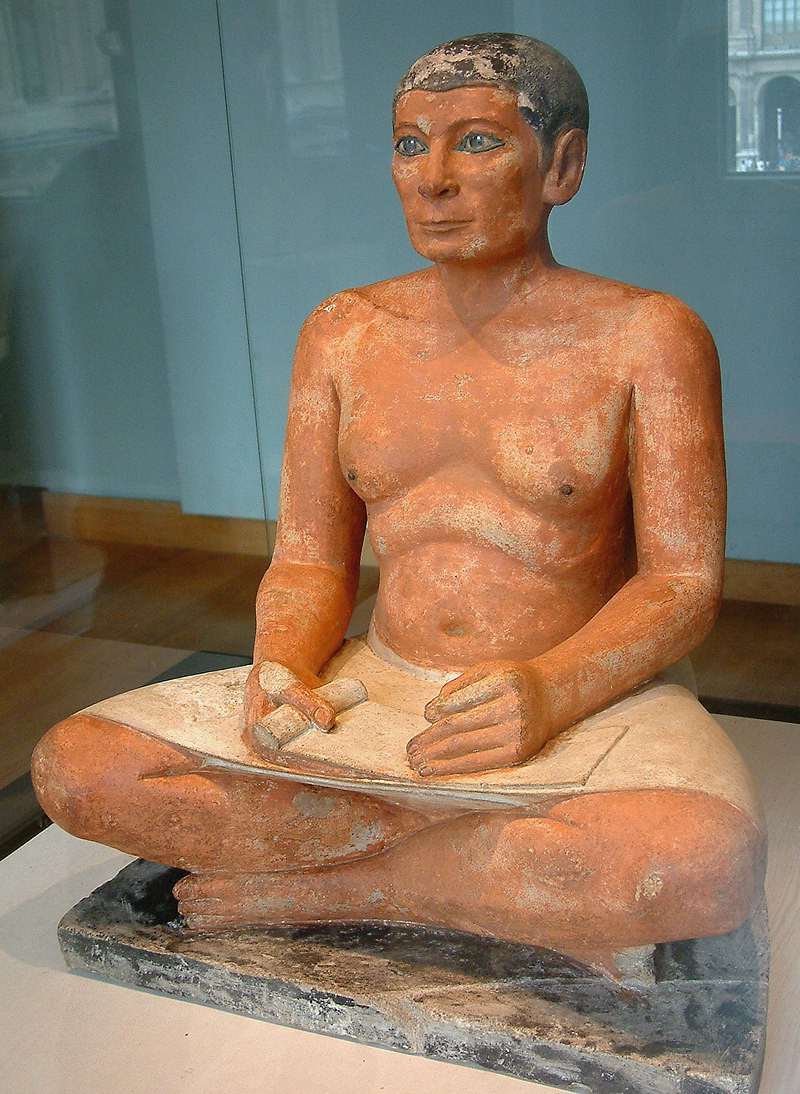
\includegraphics[height=\textheight]{./IMG/Egypte_louvre_285_scribe.jpg}
\end{center}

\end{multicols}

\vfill
\pagebreak

	\begin{center}
	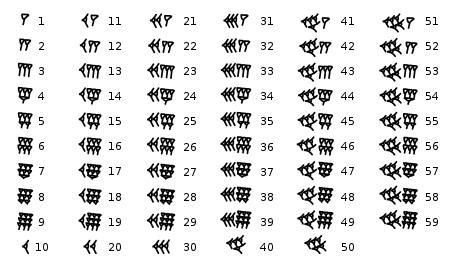
\includegraphics[height=\textheight]{./IMG/Babylonian_numerals.svg.png}
\end{center}

\vfill
\pagebreak
	
	\subsection[O Código de Hamurabi]{O Código de Hamurabi}
\begin{multicols}{2}
	\begin{center}
	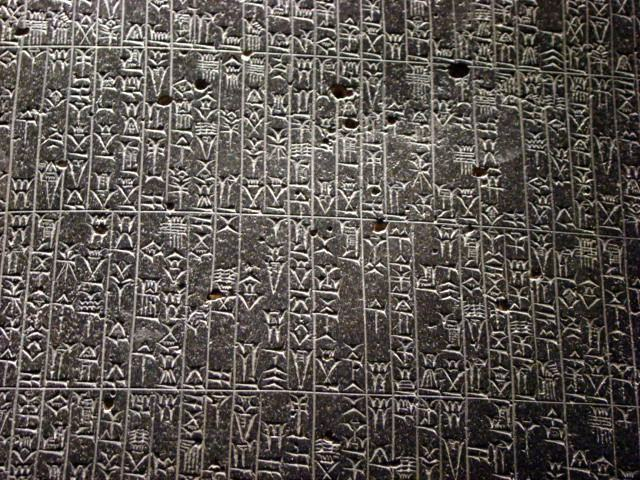
\includegraphics[width=\linewidth]{./IMG/codigo-de-hamurabi.jpg}
\end{center}	
	\vfill
	\columnbreak
	
	\begin{center}
		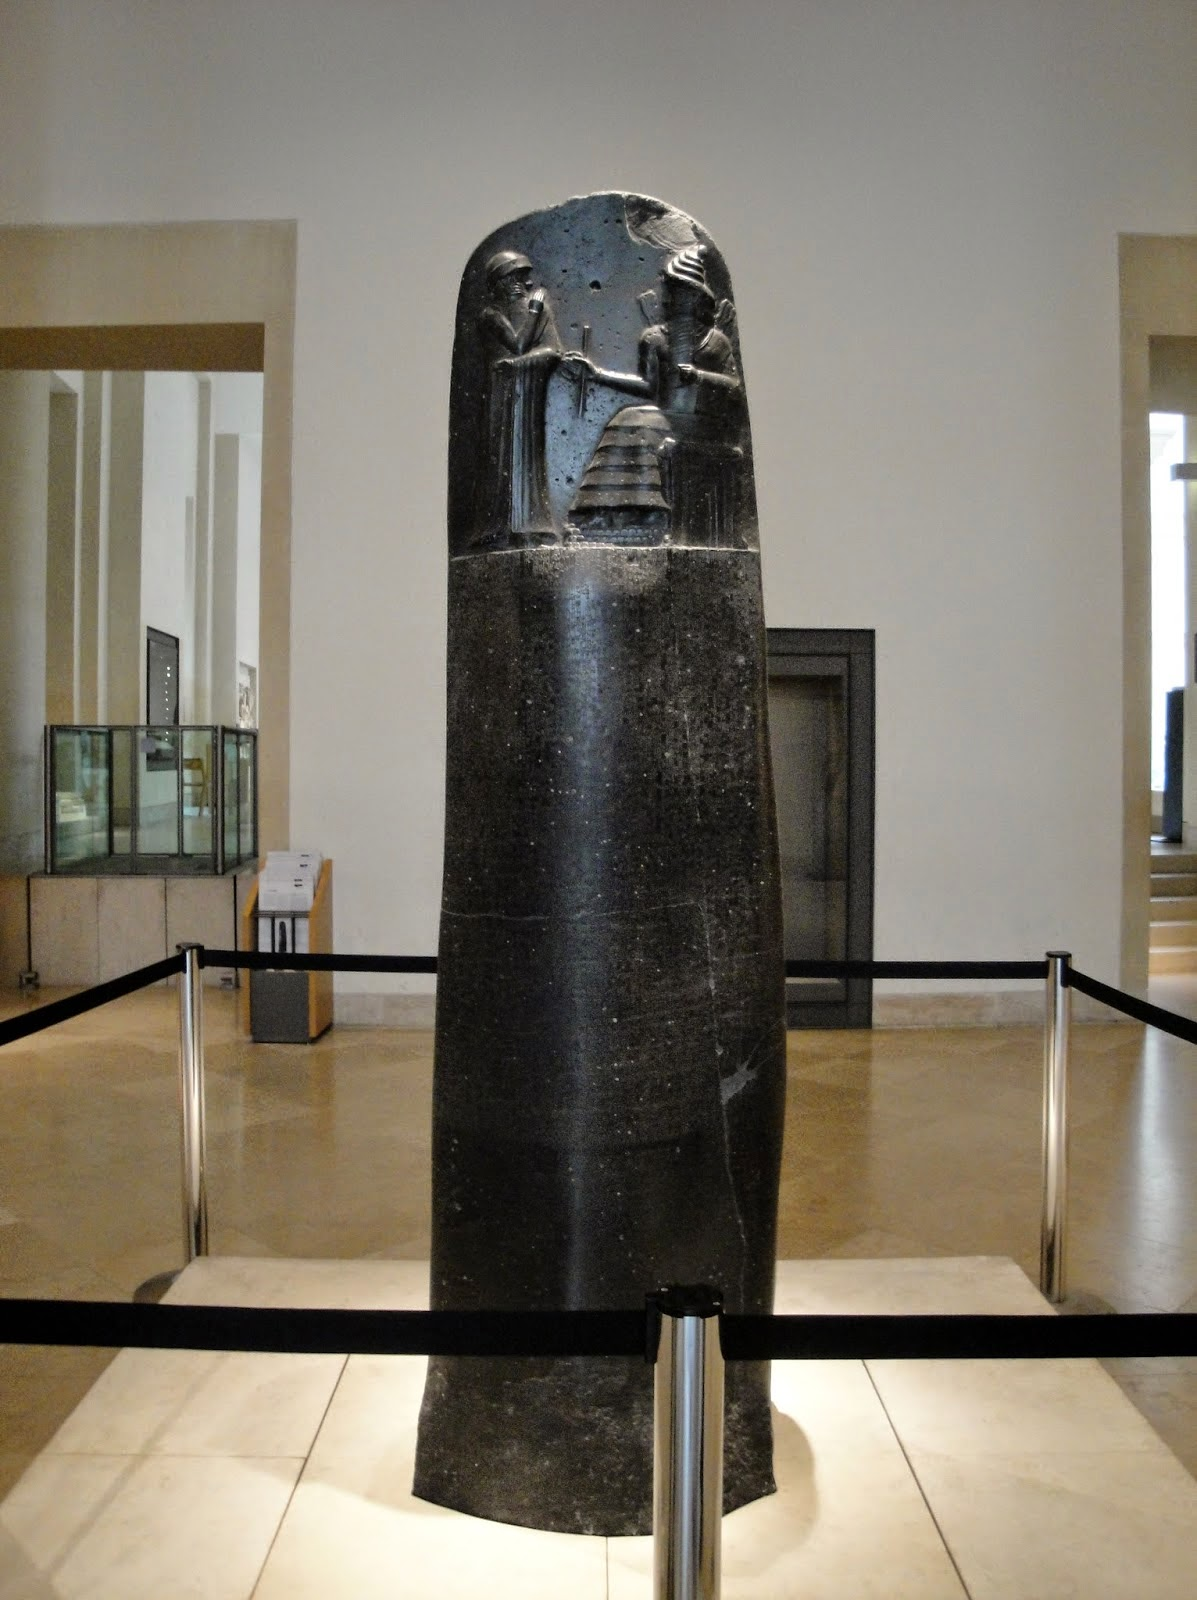
\includegraphics[height=.8\textheight]{./IMG/codigo de hamurabi.JPG}
	\end{center}

	\vfill
\columnbreak

{\Large $\sim$1754 A.C.}

{\large

\begin{itemize}
	\item Lei de Talião (olho por olho, dente por dente):

{\normalsize \subitem Punição proporcional ao crime.}

\item Responsabilidade individual:

{\normalsize \subitem Pune tanto o culpado quanto sua família se estiverem envolvidos no crime.}

\item Presunção de inocência:

{\normalsize \subitem Quem acusa deve provar.}

\item Leis relacionadas à propriedade:

{\normalsize \subitem Contratos, transações comerciais e propriedade, penas para roubo e falsificação.}

\item Questões familiares:

{\normalsize \subitem Questões familiares, como casamento, divórcio e herança.}

\item Leis de comércio:

{\normalsize \subitem Regulamentos para atividades comerciais, estabelecendo padrões e punições para práticas desonestas.}

\item Leis trabalhistas:

{\normalsize \subitem Relações de trabalho, salários e penalidades para trabalhadores que não cumpram seus deveres.}

\item Leis religiosas:

{\normalsize \subitem Práticas religiosas e rituais, indicando a influência da religião na sociedade e na legislação.}

\end{itemize}}

\vfill
\columnbreak

\large

\begin{itemize}
	
	\item \textbf{Lei 196:}
		\subitem Se um homem destruir o olho de outro homem, então seu próprio olho será destruído.
	
	\item \textbf{Lei 200:}
		\subitem Se um homem arrancar o dente de outro homem, então seu próprio dente será arrancado.
		
		\vfill\null
		\columnbreak

	\item \textbf{Lei 229:}
		\subitem Se um construtor construir uma casa para alguém, mas não a fizer de forma sólida e a casa desabar, então o construtor será morto.
	
	\item \textbf{Lei 108:}
		\subitem Se um homem acusar outro homem de assassinato, mas não puder prová-lo, então aquele que fez a acusação será morto.

	
	\item \textbf{Lei 196:}
		\subitem Se um homem em um julgamento subornar testemunhas ou juízes, então ele será morto.

\end{itemize}

\end{multicols}

\vfill
\pagebreak



\subsection[Ábaco]{Ábaco}
\begin{multicols}{3}
	\large Mesopotâmia, China: $\sim$3500 a.C.
	
	\begin{center}
	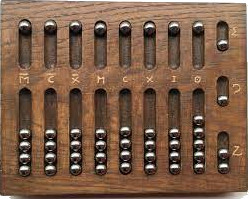
\includegraphics[width=\linewidth]{./IMG/abaco.jpeg}
\end{center}

\vfill
\columnbreak

\begin{center}
	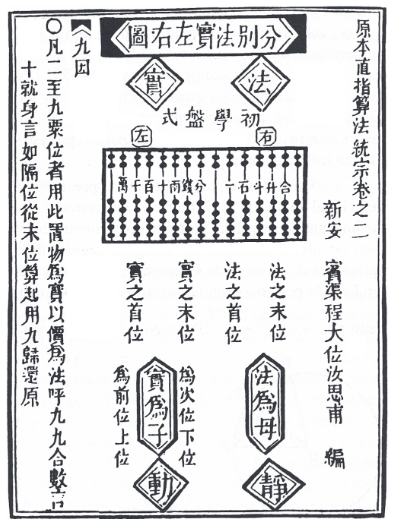
\includegraphics[width=\linewidth]{./IMG/abaco.png}
\end{center}

\vfill
\columnbreak
	
 	\begin{center}
		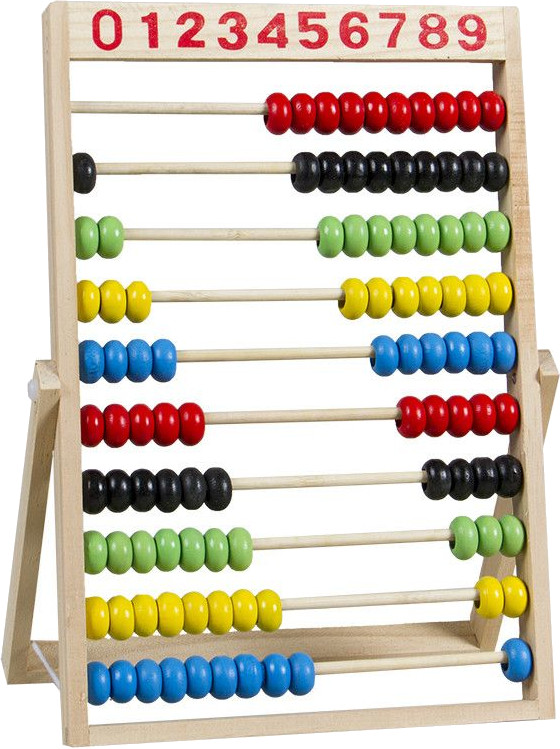
\includegraphics[width=\linewidth]{./IMG/abacus-wooden-frame-100-beads.jpg}
	\end{center}

\end{multicols}

\vfill
\pagebreak


\subsection[Velas para contar o tempo]{Velas para contar o tempo}
\large
Stonehenge: $\sim$3100 - 2075 a.C.
\begin{center}
	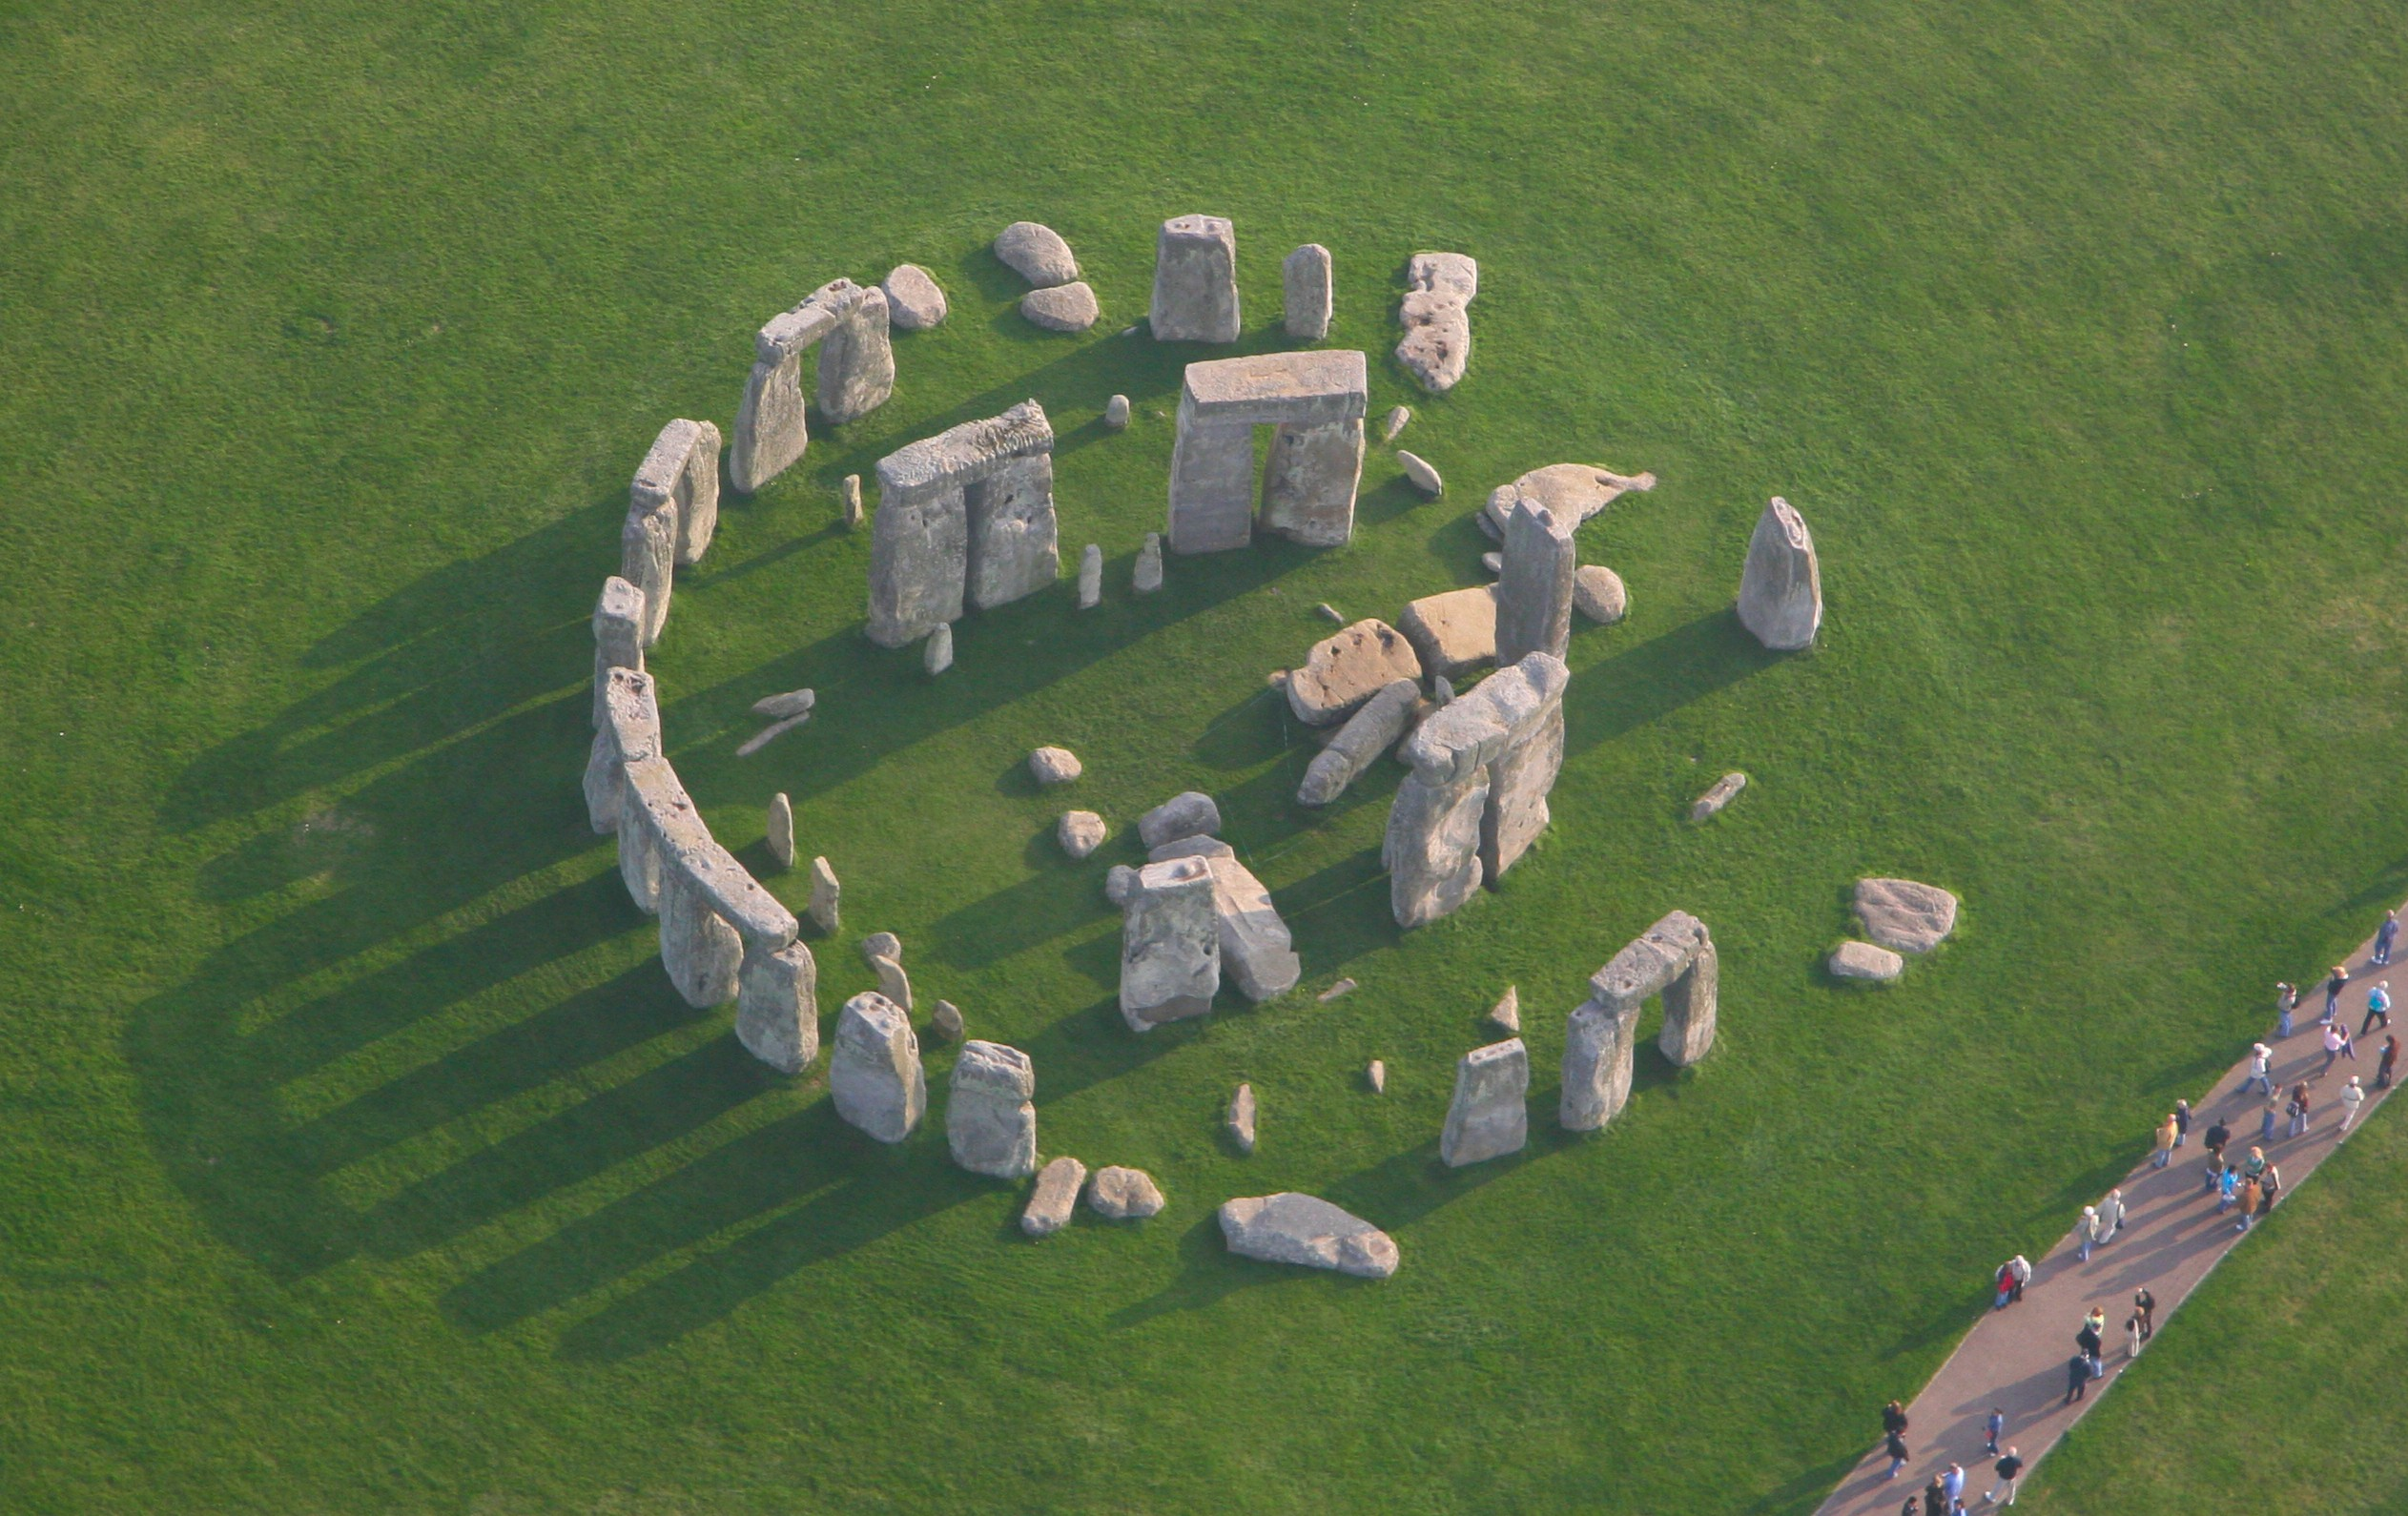
\includegraphics[height=.75\textheight]{./IMG/valuable_europe_265732.jpg}
\end{center}

\vfill
\pagebreak

\begin{multicols}{2}
	
	Relógio de sol: $\sim$1500 a.C.
	\begin{center}
		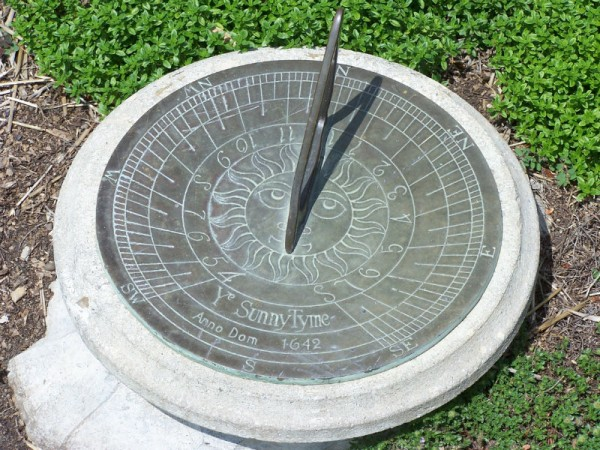
\includegraphics[width=\linewidth]{./IMG/Tempo-Relogio-de-Sol-600x450.jpg}
	\end{center}

\vfill\null
\columnbreak

Clepsidra: $\sim$1400 a.C.
	\begin{center}
	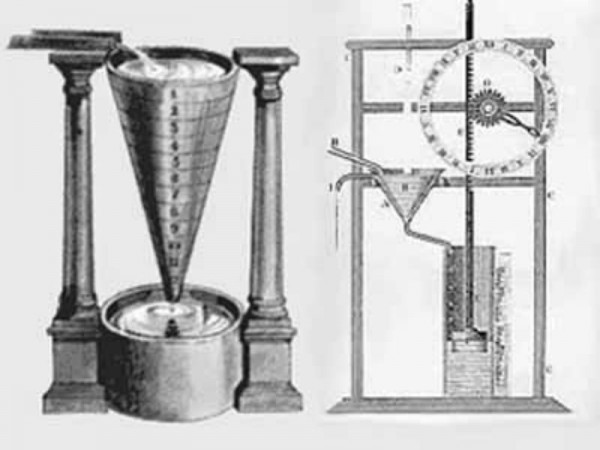
\includegraphics[width=\linewidth]{./IMG/Tempo-Clepsidra-600x450.jpg}
\end{center}

\vfill
\pagebreak
\end{multicols}

\begin{multicols}{3}

Anticítera: $\sim$séc 1 a.C.

		\begin{center}
	\includegraphics[width=\linewidth]{./IMG/NAMA_Machine_d'Anticythère_1.jpg}
\end{center}

\vfill\null
\columnbreak

\begin{center}
	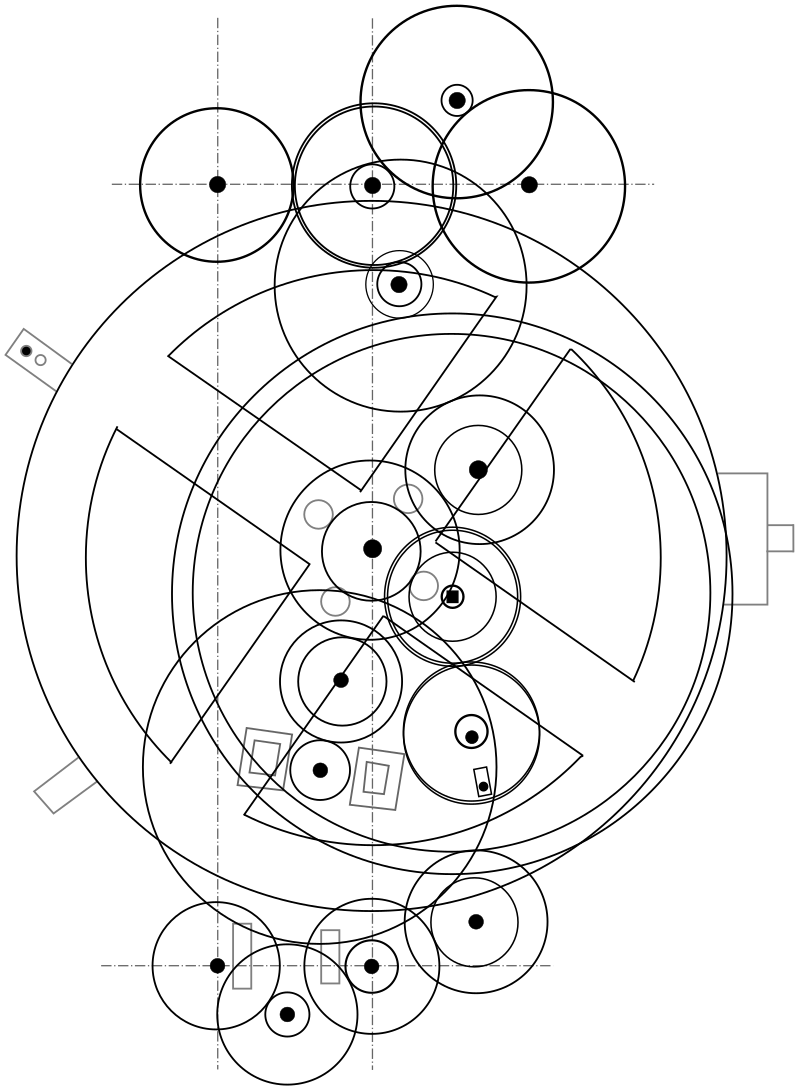
\includegraphics[width=\linewidth]{./IMG/800px-Antikythera_mechanism.svg}
\end{center}

\vfill\null
\columnbreak

\begin{center}
	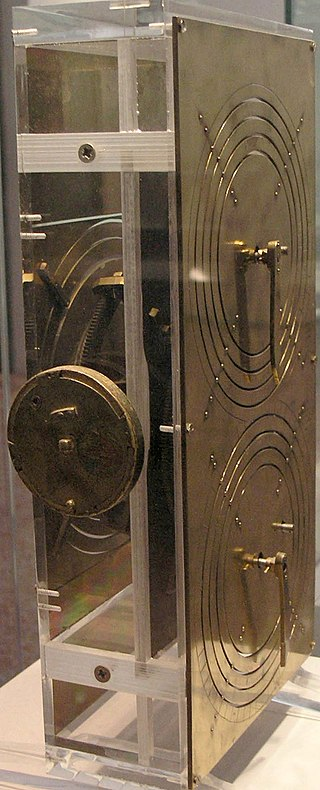
\includegraphics[width=.9\linewidth,height=\textheight]{./IMG/Anticythere.jpg}
\end{center}

\vfill
\pagebreak

Ampulheta: $\sim$sec. 7.
	\begin{center}
	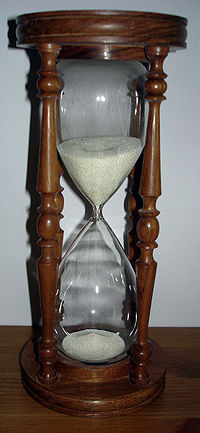
\includegraphics[height=.9\textheight]{./IMG/200px-Wooden_hourglass.jpg}
\end{center}

\vfill
\columnbreak

Relógio de vela: $\sim$sec. 8.
	\begin{center}
	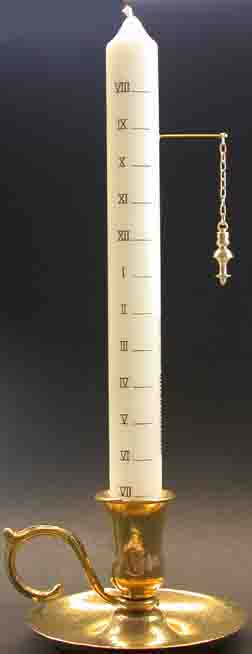
\includegraphics[height=.9\textheight]{./IMG/aeb6915395e4f1a99f80b6f692a88e22.jpg}
\end{center}

\vfill
\columnbreak

Relógio de pêndulo\\(Christiaan Huygens):  1656.

	\begin{center}
	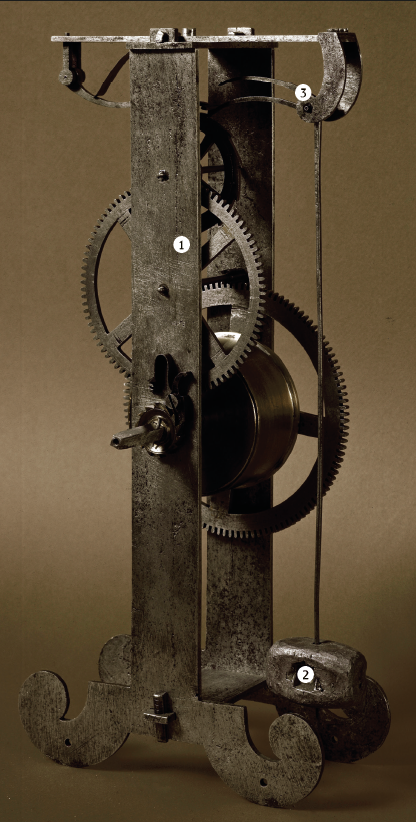
\includegraphics[height=.8\textheight]{./IMG/g8.png}
\end{center}
\end{multicols}
\vfill
\pagebreak

\begin{multicols}{2}

Relógio de quartzo (Warren Marrison): 1955.

\begin{center}
	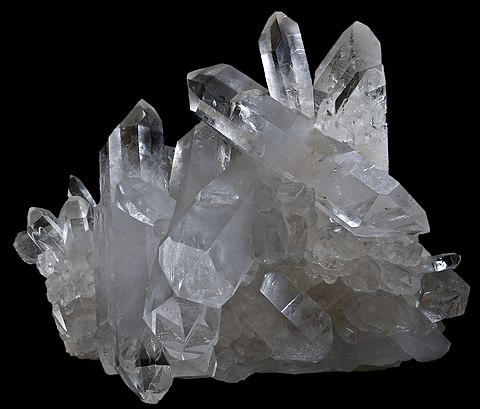
\includegraphics[height=.8\textheight]{./IMG/Quartz_Brésil.jpg}
\end{center}

\vfill
\columnbreak

\begin{center}
	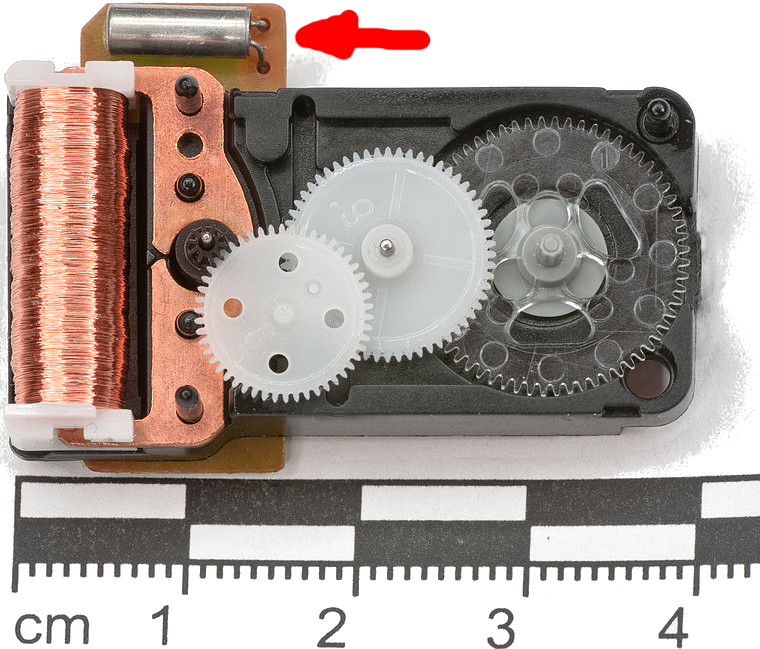
\includegraphics[width=\linewidth]{./IMG/800px-Quartz_Clockwork_(disassembled).jpg}
\end{center}

\vfill\null
\columnbreak

Relógio atômico: 1955.
	\begin{center}
	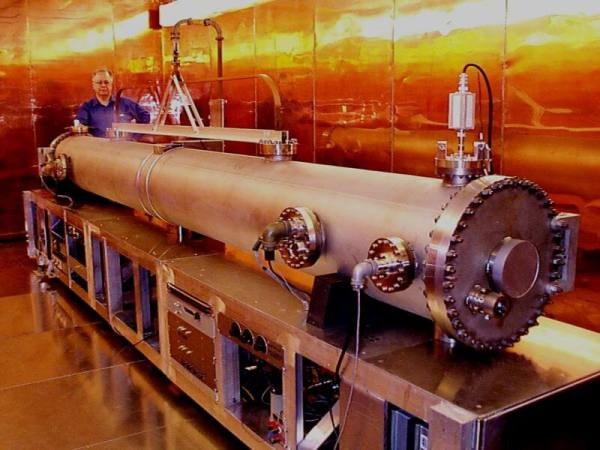
\includegraphics[width=\linewidth]{./IMG/Tempo-Relogio-Atomico-600x450.jpg}
\end{center}

\vfill
\columnbreak

\begin{center}
	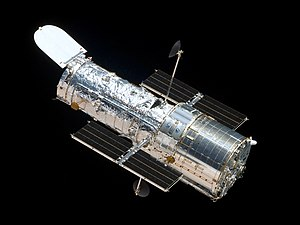
\includegraphics[width=\linewidth]{./IMG/HST-SM4.jpeg}
\end{center}
\end{multicols}

\vfill\null
\pagebreak

	
	\subsection[Tipos móveis]{Tipos móveis}
\begin{multicols}{2}
	
	Sutra Jingang, da Dinastia Tang, $\sim$sec. 8.

	\begin{center}
		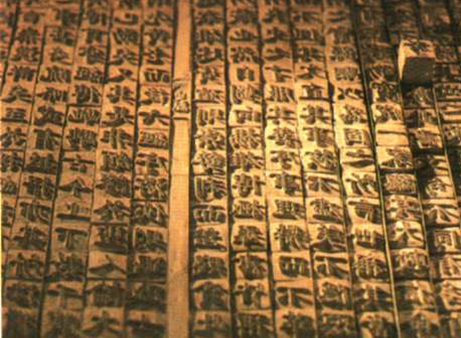
\includegraphics[width=\linewidth]{./IMG/download.png}
	\end{center}

\vfill
\columnbreak
Guttemberg: sec. 14.
	\begin{center}
		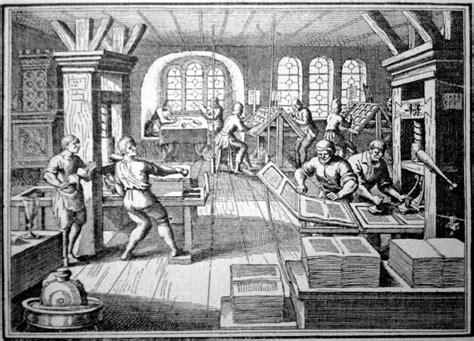
\includegraphics[width=\linewidth]{./IMG/th-620000562.jpg}
	\end{center}

\vfill
\columnbreak

	\begin{center}
	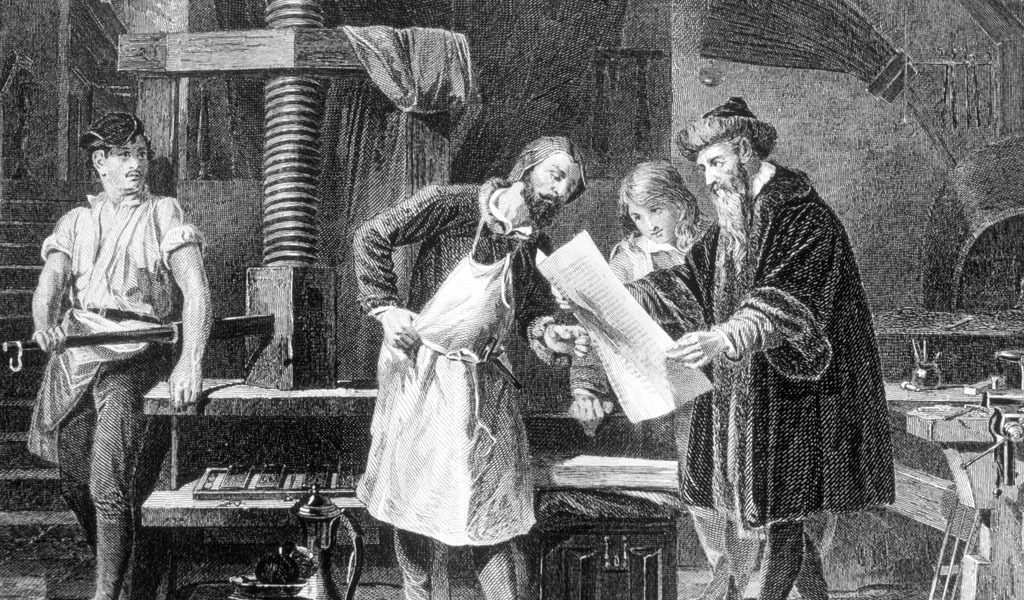
\includegraphics[width=\linewidth]{./IMG/02.jpg}
\end{center}

\vfill
\columnbreak

	\begin{center}
		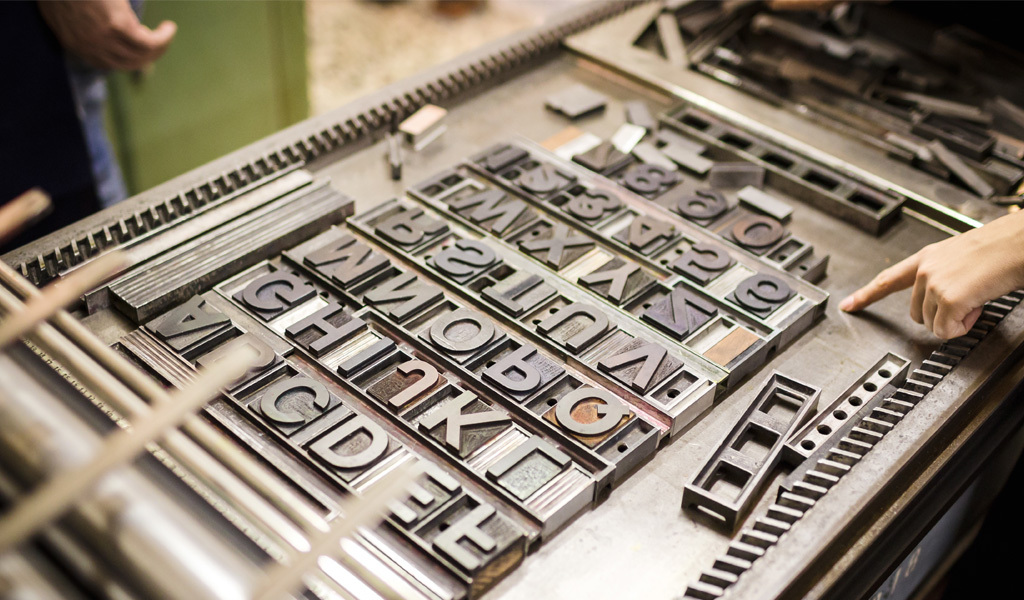
\includegraphics[width=\linewidth]{./IMG/03-1.jpg}
	\end{center}
\end{multicols}

\vfill
\pagebreak
	
	\subsection[Pascaline]{Pascaline}
\begin{multicols}{2}
	
	\begin{center}
		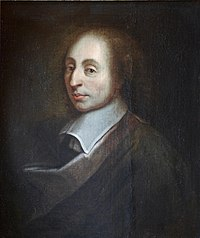
\includegraphics[height=.9\linewidth]{./IMG/Blaise_Pascal_Versailles.JPG}
	\end{center}


\vfill
\columnbreak

Em 1642 o matemático francês Blaise Pascal, que era filho de um cobrador de impostos, inventou uma máquina automática de cálculos para agilizar o trabalho do seu pai.

	\begin{center}
	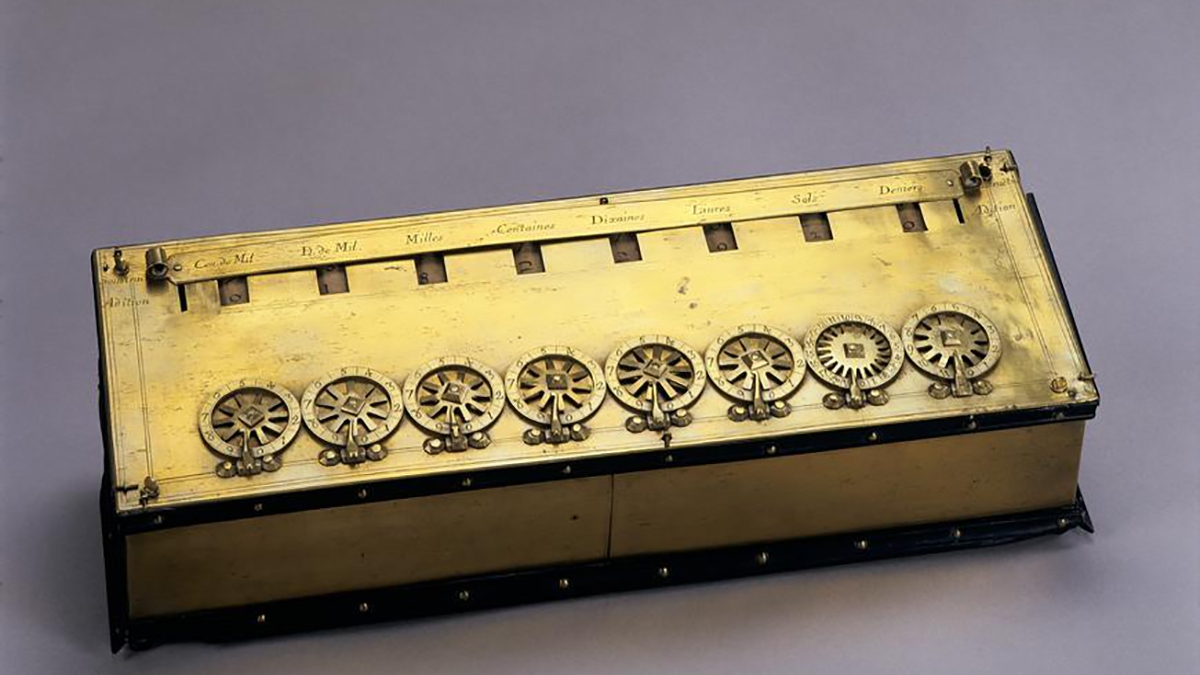
\includegraphics[width=\linewidth]{./IMG/pascaline.jpg}
\end{center}

\end{multicols}

\vfill
\pagebreak

	
%\subsection[Ossos de Napier]{Ossos de Napier}
%\vfill\null
\pagebreak


	
	\subsection[Tear]{Tear}
\large
\begin{multicols}{2}
	\begin{itemize}
		\item Revolução neolítica
		\item $\sim$ 10.000 a.C ou antes
		\item princípio da tecelagem
		\normalsize
		\begin{itemize}
		\item teias de aranha
		\item ninhos de pássaro
		\item pequenos galhos
		\item barreiras
		\item escudos
		\item cestas
		\item habitações
		\end{itemize}
		 \item Tecidos
	
	\end{itemize}
	
	\vfill\null
\columnbreak

\vspace*{-15mm}
\begin{center}
	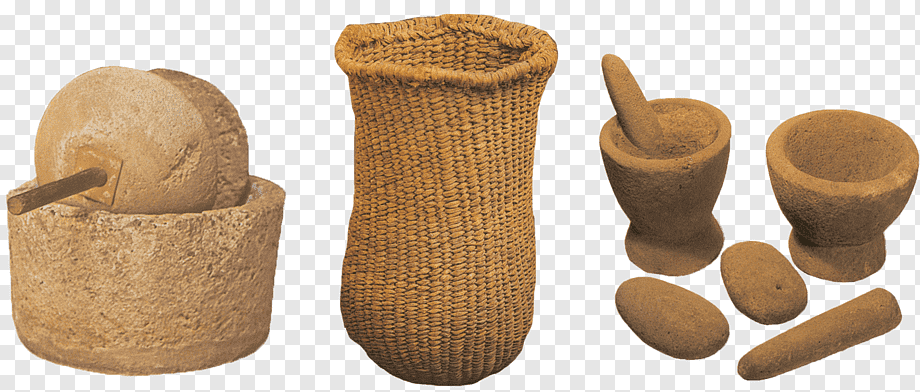
\includegraphics[width=.8\linewidth]{./IMG/png-transparent-neolithic-revolution-paleolithic-prehistory-mesolithic-homens-textile-pottery-revolution.png}
\end{center}

\begin{center}
	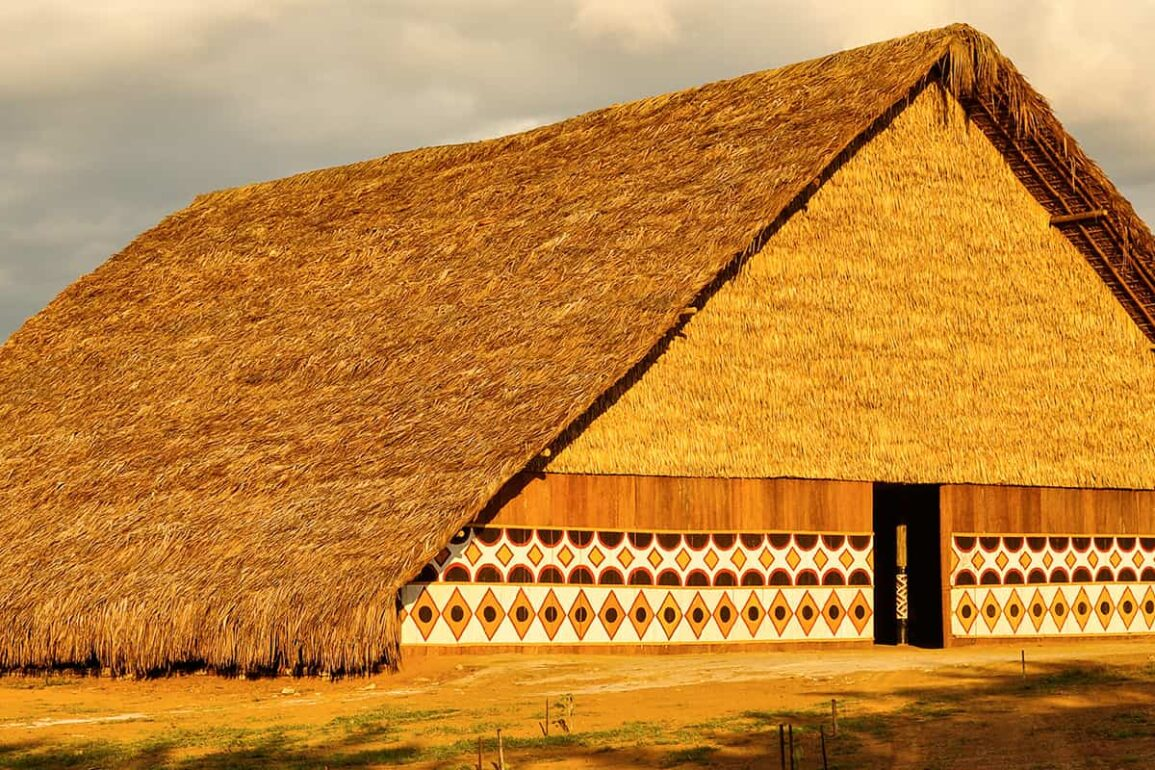
\includegraphics[width=.8\linewidth]{./IMG/revistaSIM_Arquitetura-Indigena_Destaque_Credito-Julio-Duarte_Shutterstock.com_-1155x770.jpg}
\end{center}


\vfill
\pagebreak

\begin{center}
	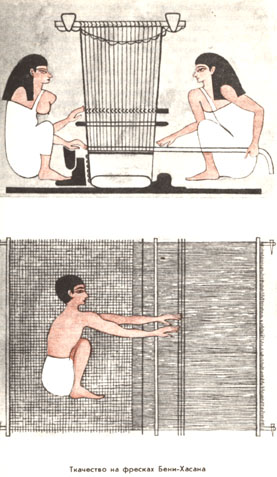
\includegraphics[height=.9\textheight]{./IMG/tear-egito.jpg}
\end{center}

\null
\columnbreak

\begin{center}
	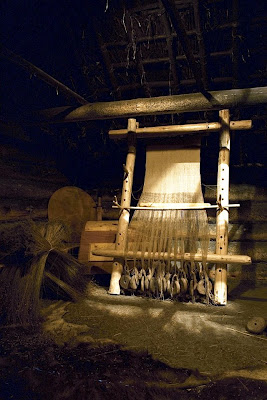
\includegraphics[height=.9\textheight]{./IMG/tear-europa.jpg}
\end{center}

\null
\columnbreak

\begin{center}
	\includegraphics[width=.9\linewidth]{./IMG/Tecer.jpg}
\end{center}

\null
\columnbreak

\begin{center}
	\includegraphics[width=.9\linewidth]{./IMG/Tecer2.jpg}
\end{center}

\end{multicols}
\vfill
\pagebreak



	
\subsection[Spinning Jenny]{Spinning Jenny}
\begin{multicols}{2}
	
	James Hargreaves (1770)
\begin{center}
	\includegraphics[height=.8\textheight]{./IMG/250px-James_Hargreaves.jpg}
\end{center}

\vfill
\columnbreak

\begin{center}
	\includegraphics[height=.9\textheight]{./IMG/M816020_How-the-Early-Spinning-Jenny-Worked.jpg}
\end{center}
\end{multicols}

\vfill
\pagebreak

\begin{center}
	\includegraphics[height=.9\textheight]{./IMG/spinninjenny.jpeg}
\end{center}


\vfill
\pagebreak

\begin{center}
	\includegraphics[height=.9\textheight]{./IMG/A003171.jpg}
\end{center}

\vfill
\pagebreak


	
	\subsection[Máquina a vapor]{Máquina a vapor}
\begin{multicols}{2}
Eolípila: Heron de Alexandria (séc. 1)	

\begin{center}
	\includegraphics[height=.8\textheight]{./IMG/Aeolipile_illustration.png}
\end{center}

\vfill
\columnbreak

\begin{center}
	\includegraphics[height=.9\textheight]{./IMG/Aeolipile.jpg}
\end{center}

\end{multicols}

\vfill
\pagebreak

James Watt (1777)

\begin{center}
	\includegraphics[width=.9\linewidth]{./IMG/20190205-maquina-vapor.jpg}
\end{center}


\vfill
\pagebreak



	\subsection[Tear a vapor]{Tear a vapor}
\begin{center}
	\includegraphics[height=.9\textheight]{./IMG/tear-mecanico.jpg}
\end{center}

\vfill
\pagebreak
	
	\subsection[Tear de Jaccqard]{Tear de Jaccqard}
\begin{center}
	\includegraphics[height=.9\textheight]{./IMG/Figura-14-Cartoes-perfurados-em-um-tear-ou-maquina-de-Jacquard.png}
\end{center}

\vfill
\pagebreak

\begin{center}
	\includegraphics[height=\textheight]{./IMG/tapete.jpeg}
\end{center}

\vfill
\pagebreak

	
	\subsection[Máquina Diferencial]{Máquina Diferencial}
\begin{multicols}{2}
	\begin{center}
		\includegraphics[height=.8\textheight]{./IMG/ada-lovelace.jpg}
	\end{center}
\end{multicols}

\vfill
\pagebreak



	\subsection[Gottfried Leibniz]{Gottfried Leibniz}
\begin{multicols}{2}
	\begin{center}
	\includegraphics[height=.9\textheight]{./IMG/Gottfried+Wilhelm+Leibniz.jpg}
	\end{center}
	
	\vfill
	\columnbreak

\begin{itemize}
	\item séc. 18
	\item Lógica binária
	\item Escrituras chinesas
\end{itemize}	
\end{multicols}

\vfill
\pagebreak

\begin{center}
	\includegraphics[height=\textheight]{./IMG/MAO-10.jpg}
\end{center}

\vfill
\pagebreak

{\Huge
Base 10
}
\vspace*{-10mm}
{
	\Large
\begin{center}
		\begin{tabular}{*{10}{r}}
	\csvreader[no head, tabular=*{9}{c}c, table head=\\]%
	{./CSV/TABELA.csv}{}%
	{\csvcoli &}%
\end{tabular}
\end{center}

}

\vfill
\pagebreak


\begin{multicols}{2}
	
	
	\begin{center}
		\includegraphics[width=\linewidth]{./IMG/argila.jpeg}
	\end{center}
	
	\vfill
	\columnbreak
	
	\begin{center}
	\includegraphics[height=.5\textheight]{./IMG/MAO-60.jpg}
	
	\includegraphics[height=.45\textheight]{./IMG/PES-60.jpg}
\end{center}
\end{multicols}

\vfill
\pagebreak

{\Huge
	Base 60
}
\begin{center}
	\includegraphics[height=.9\textheight]{./IMG/Babylonian_numerals.svg.png}
\end{center}

\vfill
\pagebreak

	\begin{center}
	\includegraphics[height=\textheight]{./IMG/cobra.jpg}
\end{center}

\vfill
\pagebreak
\begin{multicols}{2}
	
	{\LARGE
		Base Binária: 0 e 1.
	}
	
	\large "[…] não uso nenhum outro caractere além do 0 e 1, e quando chego neste segundo, eu começo de novo."
	
	{\normalsize Fonte: \href{http://www.leibniz-translations.com/binary.htm}{http://www.leibniz-translations.com/binary.htm}}
	
	
%
\ExplSyntaxOn
\foreach \dec in {0,...,15} {%
	\int_to_bin:n { \dec } \\
}
\ExplSyntaxOff

%%
	\vfill\null
	\columnbreak
	




%	
%	\ExplSyntaxOn
%	\newsavebox{\mybox}
%	\begin{lrbox}{\mybox}
%		\begin{minipage}{\linewidth}
%			\begin{tabular}{|>{\raggedleft\arraybackslash}p{1.5cm}|>{\centering\arraybackslash}p{1.5cm}|}
%				\hline
%				\textbf{Decimal} & \textbf{Binário} \\
%				\hline
%				\foreach \dec in {0,...,15} {
%					\dec & \int_to_bin:n { \dec } \\
%					\hline
%				}
%			\end{tabular}
%		\end{minipage}
%	\end{lrbox}
%	
%	\noindent\usebox{\mybox}
%	\ExplSyntaxOff
%	
	
	
	

%\newsavebox{\mybox}
%\begin{lrbox}{\mybox}
%	\begin{minipage}{\linewidth}
%		\begin{tabular}{|>{\raggedleft\arraybackslash}p{1.5cm}|>{\centering\arraybackslash}p{1.5cm}|}
%			\hline
%			\textbf{Decimal} & \textbf{Binário} \\
%			\hline
%			\ExplSyntaxOn
%			\foreach \dec in {0,...,15} {
%				\dec & \int_to_bin:n { \dec } \\
%				\hline
%			}
%			\ExplSyntaxOff
%		\end{tabular}
%	\end{minipage}
%\end{lrbox}
%
%\begin{tabular}{p{\linewidth}}
%	\usebox{\mybox}
%\end{tabular}

		\vfill
	\columnbreak
\normalsize	
%
%\begin{flushright}
%\textbf{	\begin{tabular*}{\textwidth}{@{\extracolsep{\fill}}*{3}{r}@{}}
%	\csvreader[no head, tabular=*{2}{r}r, table head=\\]%
%		{./CSV/BINARIOS.csv}{}%
%		{\csvcoli & \csvcolii & \csvcoliii}%
%	\end{tabular*}}
%\end{flushright}

\end{multicols}

\vfill
\pagebreak
{\LARGE 4 operações}
\begin{center}
	\includegraphics[height=.9\textheight]{./IMG/leibnizbinario.png}
\end{center}

\vfill
\pagebreak
	
	\subsection[George Boole]{George Boole}
\begin{multicols}{2}
	\begin{center}
		\includegraphics[height=.8\textheight]{./IMG/boole.jpg}
	\end{center}

\vfill
\columnbreak

\begin{itemize}
	\item 1849: “Análise Matemática da Lógica”
	\item Álgebra de Boole
	\item Álgebra booleana
\end{itemize}

"[...] É com base nesse princípio geral que eu pretendo estabelecer o \textbf{cálculo da lógica, e que reivindico para ele um lugar entre as formas reconhecidas da análise matemática}."

\vfill\null
\columnbreak
{\large \textbf{FALSO}\\
0\\
NÃO\\
DESLIGADO
}


\begin{center}
	\includegraphics[height=.7\textheight]{./IMG/FALSO.png}
\end{center}

\vfill
\columnbreak

{\large \textbf{VERDADEIRO}\\	
	1\\	
	SIM\\	
	LIGADO\
}

\begin{center}

	\includegraphics[height=.7\textheight]{./IMG/VERDADEIRO.png}
\end{center}

\vfill
\columnbreak

\begin{center}
	\includegraphics[width=.9\linewidth]{./IMG/Screenshot_20231216_190844.png}
\end{center}

\vfill
\columnbreak

\begin{center}
	\includegraphics[width=.9\linewidth]{./IMG/Screenshot_20231216_191027.png}
\end{center}
\end{multicols}



\begin{table}[h]
	\centering
	\Large
	\caption{\textbf{Tabela Verdade}}
	\begin{tabular}{|>{\centering\arraybackslash}p{.125\textwidth}|>{\centering\arraybackslash}p{.125\textwidth}|}
		\hline
		\textbf{Botão} & \textbf{Lâmpada} \\
		\hline
		\textbf{0} & \textbf{0} \\
		\hline
			\textbf{1} & \textbf{1} \\
		\hline
	\end{tabular}
\end{table}




\vfill
\pagebreak

\begin{multicols}{3}


\begin{center}
	\includegraphics[width=\linewidth]{./IMG/Screenshot_20231216_191616.png}
\end{center}

 
 \begin{center}
 	\includegraphics[width=\linewidth]{./IMG/Screenshot_20231216_191707.png}
 \end{center}

\vfill\null
\columnbreak

\begin{center}
	\includegraphics[width=\linewidth]{./IMG/Screenshot_20231216_191640.png}
\end{center}

\begin{center}
	\includegraphics[width=\linewidth]{./IMG/Screenshot_20231216_191745.png}
\end{center}

\vfill\null
\columnbreak

 \centering
\begin{tabular}{|>{\centering\arraybackslash}p{.25\linewidth}|>{\centering\arraybackslash}p{.25\linewidth}|>{\centering\arraybackslash}p{.25\linewidth}|}
	\hline
	A & B & L\\
	\hline
	0 & 0 & 0 \\
	\hline
	1 & 0 & 0 \\
	\hline
	0 & 1 & 0 \\
	\hline
	1 & 1 & 1 \\
	\hline
\end{tabular}

\vfill\null
\columnbreak

\begin{center}
	\includegraphics[width=.8\linewidth]{./IMG/Screenshot_20231216_192237.png} 
\end{center}
   
\begin{center}
	\includegraphics[width=.8\linewidth]{./IMG/Screenshot_20231216_192323.png}
\end{center}

\vfill
\columnbreak
 
\begin{center}
	\includegraphics[width=.8\linewidth]{./IMG/Screenshot_20231216_192257.png}
\end{center}
    
\begin{center}
	\includegraphics[width=.8\linewidth]{./IMG/Screenshot_20231216_192355.png}
\end{center}

\vfill
\columnbreak

 \centering
\begin{tabular}{|>{\centering\arraybackslash}p{.25\linewidth}|>{\centering\arraybackslash}p{.25\linewidth}|>{\centering\arraybackslash}p{.25\linewidth}|}
	\hline
	A & B & L\\
	\hline
	0 & 0 & 0 \\
	\hline
	1 & 0 & 1 \\
	\hline
	0 & 1 & 1 \\
	\hline
	1 & 1 & 1 \\
	\hline
\end{tabular}


\end{multicols}

\vfill
\pagebreak
	
	\subsection[Telégrafo]{Telégrafo}
\vfill\null
\pagebreak


	
	\subsection[Hermman Hollerith]{Hermman Hollerith}
\vfill\null
\pagebreak



	\subsection[Relay]{Relay}
\vfill\null
\pagebreak


	
	\subsection[TELEX]{TELEX}
\vfill\null
\pagebreak



	\subsection[Válvula]{Válvula}
\vfill\null
\pagebreak


	
	\subsection[Conrad Zuse]{Conrad Zuse}
\vfill\null
\pagebreak


	
	\subsection[A máquina Enigma]{A máquina Enigma}
\vfill\null
\pagebreak


	
	\subsection[Alan Turing]{Alan Turing}
\begin{multicols}{2}
	\begin{center}
		\includegraphics[height=.8\textheight]{./IMG/Alan_Turing_Aged_16.jpg}
	\end{center}

\vfil\null
\columnbreak
	\begin{center}
	\includegraphics[height=.8\textheight]{./IMG/turing.jpg}
\end{center}
\vfill\null
\pagebreak

\end{multicols}

	\begin{center}
	\includegraphics[width=.9\linewidth]{./IMG/nota-turing.jpeg}
\end{center}
	
	\subsection[ENIAC]{ENIAC}
\begin{center}
	\includegraphics[height=.9\textheight]{./IMG/ENIAC.jpg}
\end{center}

\vfill
\pagebreak


	\subsection[EDVAC]{EDVAC}
\vfill\null
\pagebreak


	
	\subsection[Tansistor]{Tansistor}
\vfill\null
\pagebreak


	
	\subsection[Mainframes]{Mainframes}
\vfill\null
\pagebreak


	
	\subsection[A linguagem C]{A linguagem C}
\vfill\null
\pagebreak


	
	\subsection[UNIX]{UNIX}
\vfill\null
\pagebreak


	
	\subsection[ARPANET]{ARPANET}
\vfill\null
\pagebreak


	
\subsection[XEROX]{XEROX}
\vfill\null
\pagebreak


	
	\subsection[Video Game]{Video Game}
\begin{multicols}{2}
\large	
	Em 1958, o físico americano William Higinbotham (1910-1994) cria o primeiro videogame do mundo: \textbf{Tenis for Two}.
	
	\begin{flushright}
		\normalsize Fonte: \href{https://warpzone.me/primeiro-videogame-do-mundo-comemora-60-anos/}{https://warpzone.me/primeiro-videogame-do-mundo-comemora-60-anos/}
	\end{flushright}

\vfill\null
\columnbreak

	\begin{center}
		\includegraphics[width=\linewidth]{./IMG/tenis1-696x392.jpg}
	\end{center}

\vfill\null
\columnbreak

\begin{center}
	\includegraphics[width=\linewidth]{./IMG/tenis2.jpg}
\end{center}


\vfill\null
\columnbreak

\begin{center}
	\includegraphics[width=\linewidth]{./IMG/tenis-3.jpg}
\end{center}

\vfill\null
\columnbreak


\Large \textbf{Atari}: a lenda!

	\begin{center}
	\includegraphics[width=\linewidth]{./IMG/atari-2600-handheld-pic3-2222881701.jpg}
\end{center}

\vfil\null
\columnbreak

	\begin{center}
	\includegraphics[width=\linewidth]{./IMG/ATARI-1124950375.jpg}
\end{center}

\vfil\null
\pagebreak

\pagecolor{black}
{\color{white}Enduro}

	\begin{center}
	\includegraphics[width=\linewidth]{./IMG/enduroatari2600image1111.jpg}
\end{center}

\vfil\null
\columnbreak

{\color{white}Pacman}
\begin{center}
	\includegraphics[width=\linewidth]{./IMG/maxresdefault.jpg}
\end{center}

\end{multicols}

\vfil\null
\pagebreak

\pagecolor{white}

	\subsection[IBM PC-XT]{IBM PC-XT}
\begin{multicols}{2}
	
		\begin{center}
	\includegraphics[height=.9\textheight]{./IMG/IBM_PC_XT_IMG_0502.jpg}
\end{center}

\vfill
\columnbreak

		\begin{center}
	\includegraphics[height=.9\textheight]{./IMG/309684611_437656465127036_2827131187209411270_n.jpg}
\end{center}

\end{multicols}
\vfill
\pagebreak



	\subsection[MS-DOS]{MS-DOS}
\begin{center}
	\includegraphics[height=.9\textheight]{./IMG/MSDOS-3247283636.jpg}
\end{center}

\vfill
\pagebreak

\begin{center}
	\includegraphics[height=\textheight]{./IMG/th-2938318034.jpg}
\end{center}

\vfill
\pagebreak

	\begin{center}
	\includegraphics[height=\textheight]{./IMG/960x540-989094356.jpg}
\end{center}

\vfill
\pagebreak

\begin{center}
	\includegraphics[height=\textheight]{./IMG/MSDOS200-DISKS.jpg}
\end{center}

\vfill
\pagebreak

	\begin{center}
	\includegraphics[height=\textheight]{./IMG/screen_crop.jpeg}
\end{center}

	\vfill
\pagebreak

\begin{center}
	\includegraphics[height=\textheight]{./IMG/th-1741626982.jpg}
\end{center}

\vfill
\pagebreak

	\begin{center}
		\includegraphics[height=\textheight]{./IMG/th-3913457146.jpg}
	\end{center}
	
\vfill
\pagebreak


	
	\subsection[Apple]{Apple}
\begin{multicols}{2}
	\begin{center}
		\includegraphics[height=.9\textheight]{./IMG/jobs.jpg}
	\end{center}

\vfill
\columnbreak
	\begin{center}
	\includegraphics[height=.9\textheight]{./IMG/woz.jpg}
\end{center}

\vfill
\pagebreak	
\end{multicols}

	\begin{center}
	\includegraphics[height=\textheight]{./IMG/312582987_209249291451882_2562526748956703228_n.jpg}
\end{center}

\vfil
\pagebreak


\begin{center}
	\includegraphics[height=\textheight]{./IMG/steve-jobs-lisa-800x546.jpeg}
\end{center}

\vfill
\pagebreak
	
	\subsection[Micro\$soft Windows]{Micro\$soft Windows}
\vfill\null
\pagebreak


	
	\subsection[Richard Mathew Stallman]{Richard Mathew Stallman}
\begin{multicols}{2}

	\begin{center}
		\includegraphics[height=.8\textheight]{./IMG/rms.jpg}
	\end{center}
		
\end{multicols}
\vfill\null
\pagebreak


	
	\subsection[Linus Torlvald]{Linus Torlvald}
\vfill\null
\pagebreak


	
	\subsection[O Iphone]{O Iphone}
\vfill\null
\pagebreak


	
	\subsection[Red Hat]{Red Hat}
\vfill\null
\pagebreak


	
	\subsection[Google]{Google}
	\begin{center}
		\includegraphics[height=.75\textheight]{./IMG/google-1997.jpg}\\ (1997).
	\end{center}

\vfil\null
\pagebreak


	
	\subsection[Android]{Android}
\vfill\null
\pagebreak


	
	\subsection[Arduino]{Arduino}
\vfill\null
\pagebreak


	
	\subsection[Impressora 3D]{Impressora 3D}
\vfill\null
\pagebreak


\subsection[Robótica]{Robótica}
\vfill\null
\pagebreak


	
\subsection[Inteligência Artificial]{Inteligência Artificial}
\vfill\null
\pagebreak



\chapter[Como funciona o computador]{Como funciona o computador}

\section[O computador por dentro]{O computador por dentro}
\vfill\null
\pagebreak



\section[Software e Hardware]{Software e Hardware}
\vfill\null
\pagebreak



\section[Entrada, processamento e saída]{Entrada, processamento e saída}
\vfill\null
\pagebreak



\section[O que é um programa]{O O que é um programa}
\vfil\null
\pagebreak



\section[Bits e Bytes]{Bits e Bytes}
Para entendermos o que é um Bit e um Byte primeiro precisamos entender como a informação é gravada no HD.

Imagens em microscopio de CD/HD

\vfil\null
\pagebreak

\pagecolor{black}

\color{white}

\Huge Bit = BInary digiT

\begin{itemize}
	\item Menor unidade de informação
	\item Digito binário
	\item Ligado (1) $\mid\mid$ Desligado (0)
\end{itemize}

\begin{center}
	\resizebox{125mm}{50mm}{{\color{white}$\fullmoon\newmoon$}}
\end{center}

\vfil\null
\pagebreak
\pagecolor{white}


\section[O Código ASCII]{O Código ASCII}
\vfill\null
\pagebreak



\section[Tudo é arquivo]{Tudo é arquivo}
\vfil\null
\pagebreak



\section[Estrutura de disco e partições]{Estrutura de disco e partições}
\vfill\null
\pagebreak



\subsection[I am Root]{I am Root}
\vfill\null
\pagebreak



\subsection[Árvore Windows]{Árvore Windows}
\vfill\null
\pagebreak



\subsection[Árvore Linux]{Árvore Linux}
\vfill\null
\pagebreak



\subsection[Árvore Android]{Árvore Android}
\vfill\null
\pagebreak



\section[Sistemas Operacionais]{Sistemas Operacionais}
\vfill\null
\pagebreak



\subsection[No princípio eram os relays]{No princípio eram os relays}
\vfill\null
\pagebreak



\subsection[...e fez-se o UNIX]{...e fez-se o UNIX}
\vfill\null
\pagebreak



\subsection[MS-X / MS-DOX]{MS-X / MS-DOX}
\vfill\null
\pagebreak



\subsection[MacOS-X]{[MacOS-X}
\vfill\null
\pagebreak



\subsection[Micro\$oft Windows]{Micro\$oft Windows}
\vfill\null
\pagebreak



\subsection[MiniX]{MiniX}
\input{./TeX_Comp/MINIX.tex}

\subsection[GNU]{GNU}
\vfill\null
\pagebreak



\subsection[LinuX]{LinuX}
\vfill\null
\pagebreak



\subsection[Android]{Android}
\vfill\null
\pagebreak



\subsection[GNU de Kernel Linux]{GNU de Kernel Linux}
\vfill\null
\pagebreak



\chapter[O problema das Licenças]{O problema das Licenças}

\section[Códigos]{Códigos}

\subsection[Código-fonte]{Código-fonte}
\vfill\null
\pagebreak



\subsection[Código-máquina]{Código-máquina}
\vfill\null
\pagebreak



\subsection[Licença Proprietária]{Licença Proprietaria}
\vfill\null
\pagebreak



\subsection[Licença Livre]{Licença Livre}
\vfill\null
\pagebreak



\subsubsection[As 4 Liberdades Fundamentais do Software Livre]{As 4 Liberdades Fundamentais do Software Livre}
\vfill\null
\pagebreak



\chapter[\large O Sistema Operacional]{O Sistema Operacional}

\section [\large O UNIX]{O UNIX}

\section[M-DOS]{M-DOS}

\section[MAC]{MAC}

\section[GNU]{GNU}

\section[Linux]{Linux}

\section[GNU de Kernel Linux]{GNU de Kernel Linux}

\subsection[O que é Kernel]{O que é Kernel}

\subsubsection[O Boot]{O Boot}

\begin{itemize}
	\item BIOS
	\item Disco
	\subitem Partição
	\subsubitem Kernel
	\subitem SISTEMA OPERACIONAL
	\subsubitem Shell
	\subitem Desktop
	\item Distro
	\subitem hurd
	\subitem Slackware (u can't hack if you don´t slack!)
	\subitem Debian
	\subitem Red Hat
\end{itemize}

\subsubsection[O Boot]{O Boot}

\vfill \null\pagebreak

	
	% Adiciona referências bibliográficas
	\bibliography{suas-referencias.bib}
	
	% Fim do documento
\end{document}
